\documentclass[12pt,a4paper,twoside]{article}
\usepackage{labor}
\begin{document}

%fill for cover and header creation
\newcommand\laboratorynumber{2}
\title{Erneuerbare Energien}
\newcommand\supervisor{Ditlbacher, Harald}
\newcommand\groupnumber{42}

\newcommand\participantonelastname{Eisner}
\newcommand\participantonefirstname{Nico}
\newcommand\participantoneid{12214121}
\newcommand\participanttwolastname{Waldl}
\newcommand\participanttwofirstname{Philip}
\newcommand\participanttwoid{12214120}
\author{\participantonelastname \ \& \participanttwolastname}

\newcommand\degreeid{UB 033 678}
\newcommand\semester{23WS}
\date{10.11.2023}

%select correct course title
%\newcommand\coursetitle{Einführung in die \\ physikalischen Messmethoden}
%\newcommand\coursetitle{Laborübungen 1: \\ Mechanik und Wärme}
\newcommand\coursetitle{Laborübungen 2: \\ Elektrizität, Magnetismus, Optik}
%\newcommand\coursetitle{Fortgeschrittenen Praktikum 1: \\ Technische Physik}
%\newcommand\coursetitle{Fortgeschrittenen Praktikum 2: \\ Allgemeine Physik}

%\begin{titlepage}
   \begin{center}
       \begin{figure}[H]
            \begin{minipage}[h]{30mm}
                \centerline{
\includegraphics[height=15mm]{cover_nudes/tugraz.png}}
            \end{minipage}
            \hfill
            \begin{minipage}[h]{30mm}
                \centerline{
\includegraphics[height=15mm]{cover_nudes/nawi_graz.png}}
            \end{minipage}
            \hfill
            \begin{minipage}[h]{30mm}
                \centerline{
\includegraphics[height=15mm]{cover_nudes/uni-graz.png}}
            \end{minipage}
        \end{figure}
        
        \large{\emph{Institut für Experimentalphysik der Technischen Universität Graz \\
        \& Institut für Physik der Universität Graz}} \\
        \vspace{5mm}
        
        {\Huge \textbf{\coursetitle}}
        \vspace{5mm}
        
        {\huge \laboratorynumber: \thetitle}
    \end{center}
    
    \vfill
    
    \begin{table}[H]
        \LARGE
        \centering
        \begin{tabular}{r l}
            Betreuer:       & \supervisor \\
            Gruppennummer:  & \groupnumber \\
            \\
            Name:           & \participantonelastname, \participantonefirstname \\
            Matrikelnummer: & \participantoneid \\
            Name:           & \participanttwolastname, \participanttwofirstname \\
            Matrikelnummer: & \participanttwoid \\
            \\
            Kennzahl:       & \degreeid \\
            Datum:          & \semester \ | \thedate
        \end{tabular}
    \end{table}
    \vspace{4cm}
\end{titlepage}
\clearpage
\setcounter{page}{1}

%\maketitle %short title alternative

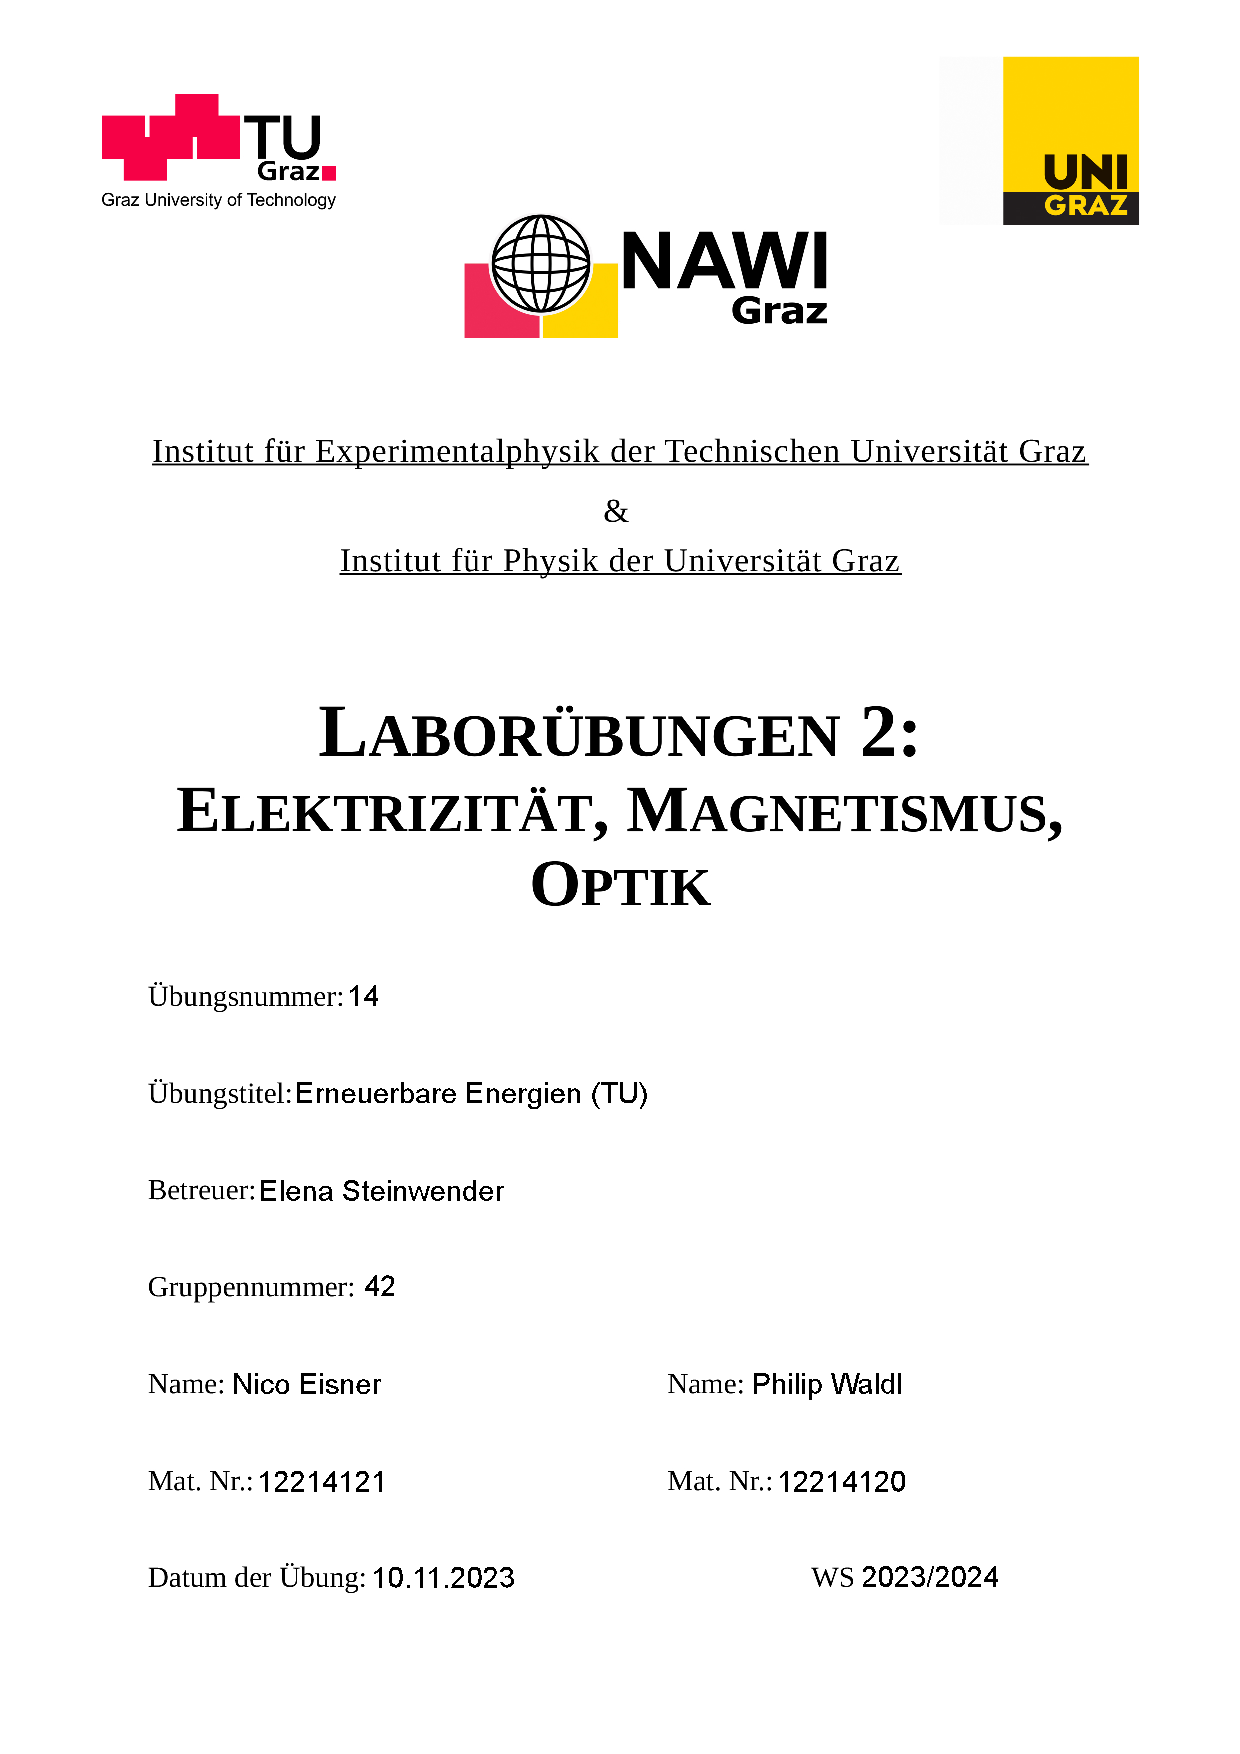
\includepdf[pages={1}]{../Deckblätter/Deckblatt_Erneuerbare_Energie.pdf}

\tableofcontents
\newpage

\section{Aufgabenstellung} %jo beschreibn wos gmocht host ------------------------------
Der Versuch Erneuerbare Energien besteht aus mehreren verschiedenen Teilen, wo mit unterschiedlichen Methoden zur Energieerzeugung gearbeitet wird. 

\subsection{Photovoltaik}
Im ersten Teilversuch gilt es mithilfe zweier Solarmodule und einer Lampe, welche als Sonne dient, verschiedene Schaltungstypen zu Testen und die Leerlaufspannung und den Kurzschlussstrom zu ermitteln. \\
Im weiteren Teil wird das selbe für unterschiedliche Abstände zur Lichtquelle wiederholt. 
\subsection{Brennstoffzelle}
Bei dem Teil der Brennstoffzelle wird an die Zelle Spannung angelegt und gemessen, ab welcher Spannung sich die Gastanks zu füllen beginnen. \\
Im zweiten Teil mit der Brennstoffzelle gilt es den Wirkungsgrad zu bestimmen. Dazu wird die Volumensänderung pro Zeit im Gastank gemessen. \\
Beim dritten Teil wird die Kennlinie der Brennstoffzelle ermittelt. Durch schrittweises verringern des Widerstandes an einem Potentiometer lässt sich die Spannung und der Strom messen und daraus die Leistung berechnen. 

\subsection{Windkraft}
Im ersten Teil wird eine Windmaschine vor ein Windrad gestellt und mit unterschiedlichen Eingangsspannungen wird die Leerlaufspannung am Windrad gemessen. 
Anschließend wird die Eingangsspannungen an der Windmaschine fixiert und das Windrad in gewissen Abständen davon entfernt und erneut die Leerlaufspannung gemessen. \\
Im zweiten Teil wird Beobachtet, was bei einzelnen Extremfällen passiert. Dazu wird der Luftstrom abbrupt gestoppt und die Leerlaufspannung am Windrad wird gemessen. 
Anschließend wird der Luftstrom abbrupt gestartet und es wird erneut die Leerlaufspannung gemessen. die beiden Extremfälle werden anschließend mit einer Kapazität zwischen Windrad und Multimeter wiederholt. 
Die Energie wird in Form eines elektrischen Potentials gespeichert. 
\\
Im letzten Teil wird durch ein Windrad Energie erzeugt, welche genutzt wird um an der Brennstoffzelle Elektrolyse zu betreiben. Hierbei wird die Energie als chemisches Potential gespeichert. 
\\
\\
Alle Informationen und Methodiken wurden uns von der Technischen Universität bereitgestellt \cite{teachcenter2}. 

\section{Voraussetzungen \& Grundlagen} %Grundlagen erklären, Formeln mit erklärung
\subsection{Photovoltaik}
Eine Solarzelle wandelt Sonnenenergie (Strahlungsenergie) in elektrische Energie um. Sie besteht aus einer Photodiode, welche aus n-dotierten und p-dotierten Halbleitern besteht. 
N-dotierte Halbleiter bestehen aus Atomen mit 5 Valenzelektronen. Diese werden auf ein Gitter aus Atomen mit 4 Valenzelektronen angebracht. 
P-dotierte Halbleiter bestehen aus Atomen mit 3 Valenzelektronen, welche an das Gitter angeordnet werden. So entstehen ''Löcher''. Kombiniert man nun die beiden Halbleiter so können Elektronen aus n-dotierten Halbleitern in die freien Löcher der p-dotierten Halbleiter. 
Dadurch entsteht Ladung an der Grenzfläche der Halbleiter und erzeugen ein elektrisches Feld. Die Grenzfläche ist nun die Raumladungszone. . 
Einfallende Photonen erzeugen Elektronen und Löcher. Diese müssen an der Grenzfläche getrennt werden, somit fließt Strom. 

\subsection{Brennstoffzelle}
Eine Brennstoffzelle kann elektrischer Energie aus Wasserstoff und Sauerstoff erzeugen. 
Dieser Prozess lässt sich auch umkehren. Fügt man der Zelle el. Energie zu, so kann aus Wasser Wasserstoff und Sauerstoff erzeugt werden. 
Die Zelle besitzt eine protonenleitende Membran (PEM) und benötigt daher keine Säuren oder Laugen. 
Der Vorgang, in dem elektrische Energie aus Wasserstoff und Sauerstoff erzeugt wird nennt man kalte Verbrennung. Der reverse Prozess, wo aus el. Energie Wasserstoff und Sauerstoff erzeugt wird nennt man Elektrolyse. 
\\
\\ 
Nutzt man die Brennstoffzelle für Elektrolyse, so wird an einer Anode Wasserstoff in Protonen und Elektronen geteilt. Die Protonen reagieren an der Kathode mit Sauerstoff und Elektronen und bilden Wasser. Die Elektronen fließen an einen äußeren Stromkreis und leisten dabei elektrische Arbeit. 
\\
Für die Erzeugung von Wasserstoff wird el. Energie in das System gespeist. Wasser wird dadurch in Wasserstoff und Sauerstoff gespalten. 
\\
\\
Die Leistung $P$, welche bei Elektrolyse entsteht, wird mit folgender Formel mit Unsicherheit berechnet. 
\begin{equation}
    \label{eq:leistung}
    \centerline{$P = U*I$  \\ $\Delta P = \vert \frac{\partial }{\partial U} * \Delta U \vert + \vert \frac{\partial }{\partial I} * \Delta I \vert$}
\end{equation}

\noindent
Desweiteren wird die Energie $E$ benötigt. Sie lässt sich mit der Formel

\begin{equation}
    \label{eq:energie}
    \centerline{$E = P*t$  \\ $\Delta E = \vert \frac{\partial }{\partial P} * \Delta P \vert + \vert \frac{\partial }{\partial t} * \Delta t \vert$}
\end{equation}
\noindent
und dazugehöriger Unsicherheit berechnen.
\\
\\
Um den Wirkungsgrad $\eta$ zu berechnen benötigt man die Leistung $P$, die Energie $E$ sowie die Masse $m$. Um den Wirkungsgrad $\eta$ in Prozent anzuschreiben multipliziert man das Ergebnis nochmals mit 100.  

\begin{equation}
    \label{eq:wirkungsgrad}
    \centerline{$\eta  = \frac{P}{E_{zu}} = \frac{P}{E*\frac{m}{molmasse}}$  \\ $\Delta \eta = \vert \frac{\partial }{\partial P} * \Delta P \vert + \vert \frac{\partial }{\partial E_{zu}} * \Delta E_{zu} \vert$}
\end{equation}


\subsection{Windkraft}
Bei einem Windrad wird aus Bewegungsenergie el. Energie erzeugt. Ein Windrad ist in Rotor und Generator geteilt. Dabei unterscheidet man zwischen horizontalen und vertikalen Ausrichtungen. Bei vertikal ausgerichteten Windrädern ist die Windrichtung nicht relevant. Bei horizontalen Windrädern, wie man sie Heutzutage sieht, ist die Windrichtung entscheident. Der große Vorteil von horizontalen gegenüber Vertikalen ist der Wirkungsgrad, welcher mehr als 50\% beträgt. 
\\
Man unterscheidet bei Wind zwei arten von Strömung. Laminare, welche gleichmäßig verläuft, und nicht laminare (turbulente) Strömung. 
Ein weiterer Punkt von Strömungen ist die Einteilung in stationäre und nicht stationäre Strömung. Bei stationärer Strömung ist die Geschwindigkeit überall im Strom konstant. 

\begin{figure}[H]
    \centering
    \includegraphics[width=0.6\linewidth]{nudes/strömung.png}
    \caption{Laminare Strömung (A, B) um verschiedene Objekte. Nicht laminare Strömung (C). Entnommen aus Skriptum Erneuerbare Energien \cite{teachcenter2}}
    \label{fig:strömung}
\end{figure}

\noindent
Um zu beschreiben, wie sich die Drücke $p$ in der laminaren Strömung verhalten, verwendet man die Bernoulli-Gleichung. Dabei entspricht $\rho$ der Dichte und $u$ der Geschwindigkeit.  

\begin{equation}
    \label{eq:bernoulli}
    \centerline{$p + \frac{1}{2} \rho u^2 = p_0 = konst. $}
\end{equation}

\noindent
Für den aerodynamischen Auftrieb werden Flügel unsymmetrischer Form verwendet, welche zu unterschiedliche Strömungsgeschwindigkeiten über und unter dem Flügel führen. Von der Bernoulli-Gleichung beschrieben führt die unterschiedliche Geschwindigkeit auch zu unterschiedlichen Drücken. 

\begin{figure}[H]
    \centering
    \includegraphics[width=0.6\linewidth]{nudes/tragfläche.png}
    \caption{Aerodynamischer Auftrieb am Beispiel einer Tragfläche. Entnommen aus Skriptum Erneuerbare Energien \cite{teachcenter2}}
    \label{fig:tragfläche}
\end{figure} 

\noindent
Daraus lässt sich die Auftriebskraft $F$ berechnen. 

\begin{equation}
    \label{eq:auftriebskraft}
    \centerline{$F = (p_2 - p_1) * A \approx \frac{1}{2} \rho_L (u_1^2 - u_2^2)*A $}
\end{equation}

\noindent
Diese Tragflächen als Flügel am Windrad führen zu Drehmoment, und erzeugen dadurch am Generator Strom. 
\\
\\
Für die Auswertung wird die erzeugte Menge an Wasserstoff/Sauerstoff pro Minute benötigt. Mit der folgenden Formel lässt sich diese, sowie dessen Unsicherheit berechnen. 
\begin{equation}
    \label{eq:prominute}
    \centerline{$Menge/min = \frac{Gesamtmenge}{Gesamtzeit}$ \\ $\Delta M/min = \vert \frac{\partial }{\partial M} * \Delta M \vert + \vert \frac{\partial }{\partial t} * \Delta t \vert$}
\end{equation}

\section{Versuchsanordnung} %mit skizze kurz beschreiben ------------------------------
Der Versuch Erneuerbare Energien ist in mehrere Teilbereiche aufgeteilt. Im Ersten wird mit einer Solarzelle gearbeitet. Im Zweiten mit einer Brennstoffzelle. Der dritte Teil besteht aus Windmaschine und Windrad. 
Im letzten Abschnitt wird das Windrad und die Brennstoffzelle kombiniert. Genauere Beschreibungen des Aufbaus werden im Abschnitt Versuchsdurchführung beschrieben.

    \begin{figure}[H]
        \centering
        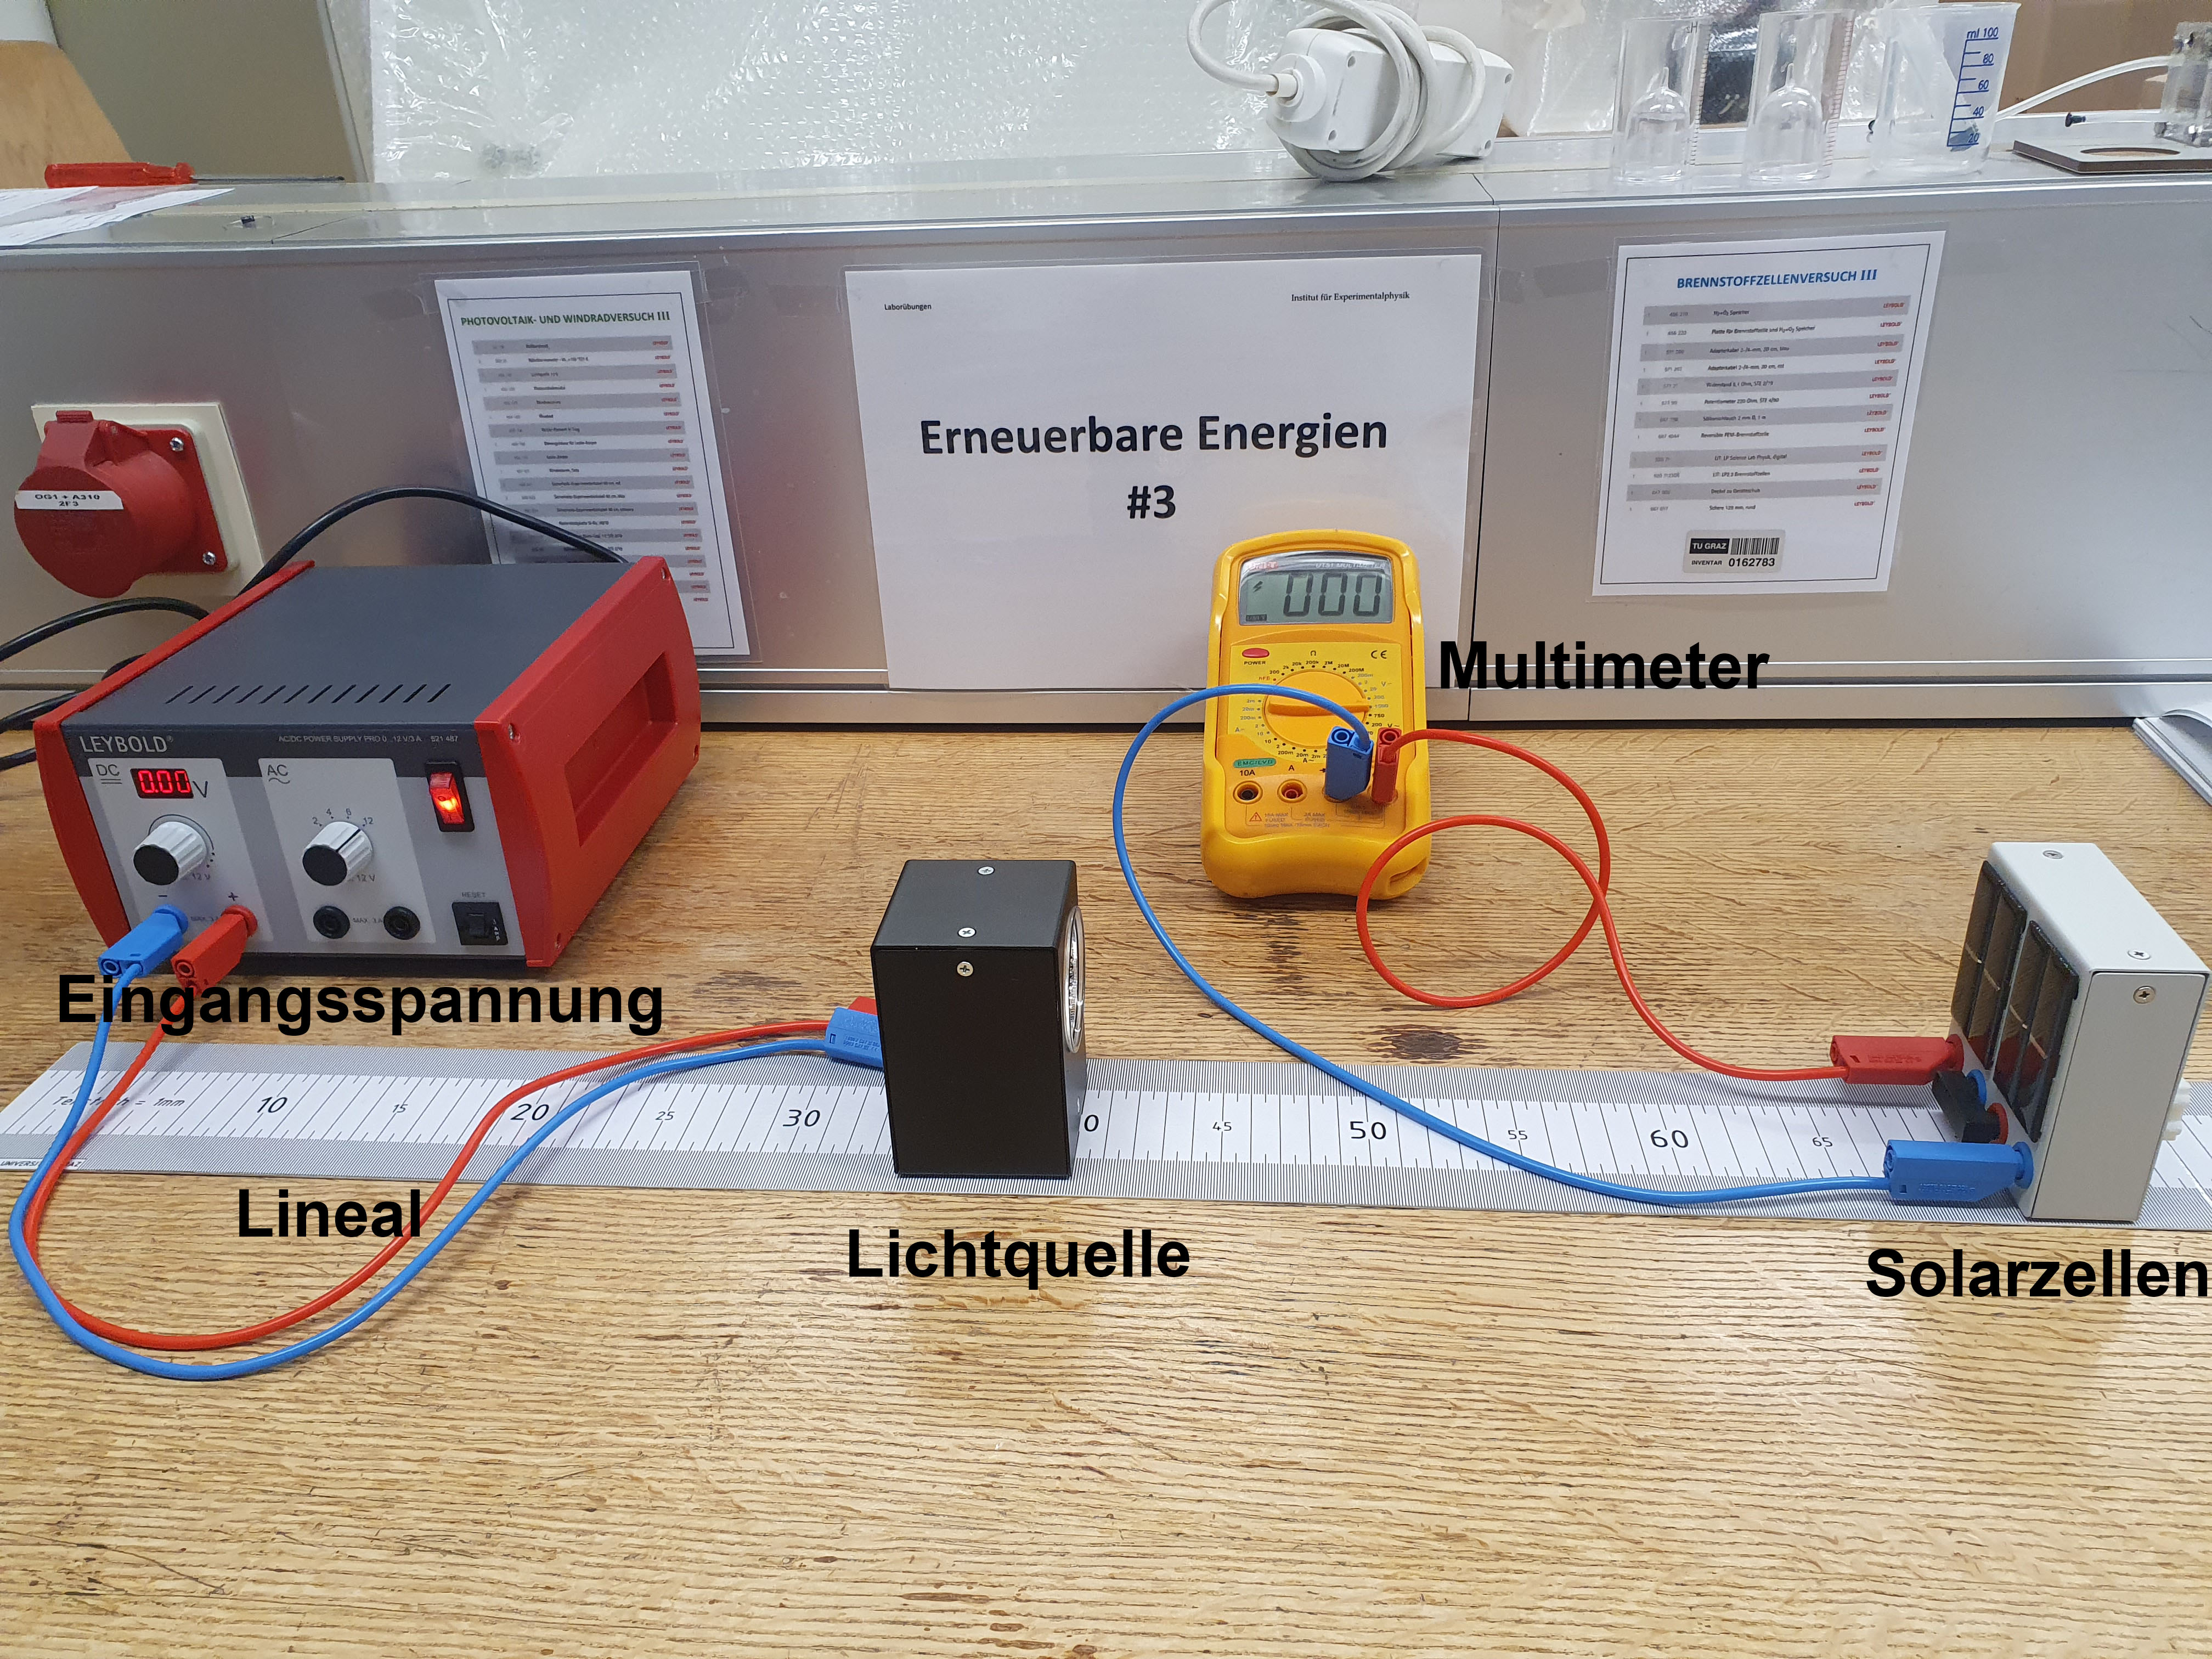
\includegraphics[width=0.6\linewidth]{nudes/solarzelle aufbau.jpg}
        \caption{Aufbau des Teilversuches Photovoltaik}
        \label{fig:aufbau Photovoltaik}
    \end{figure}

    \begin{figure}[H]
        \centering
        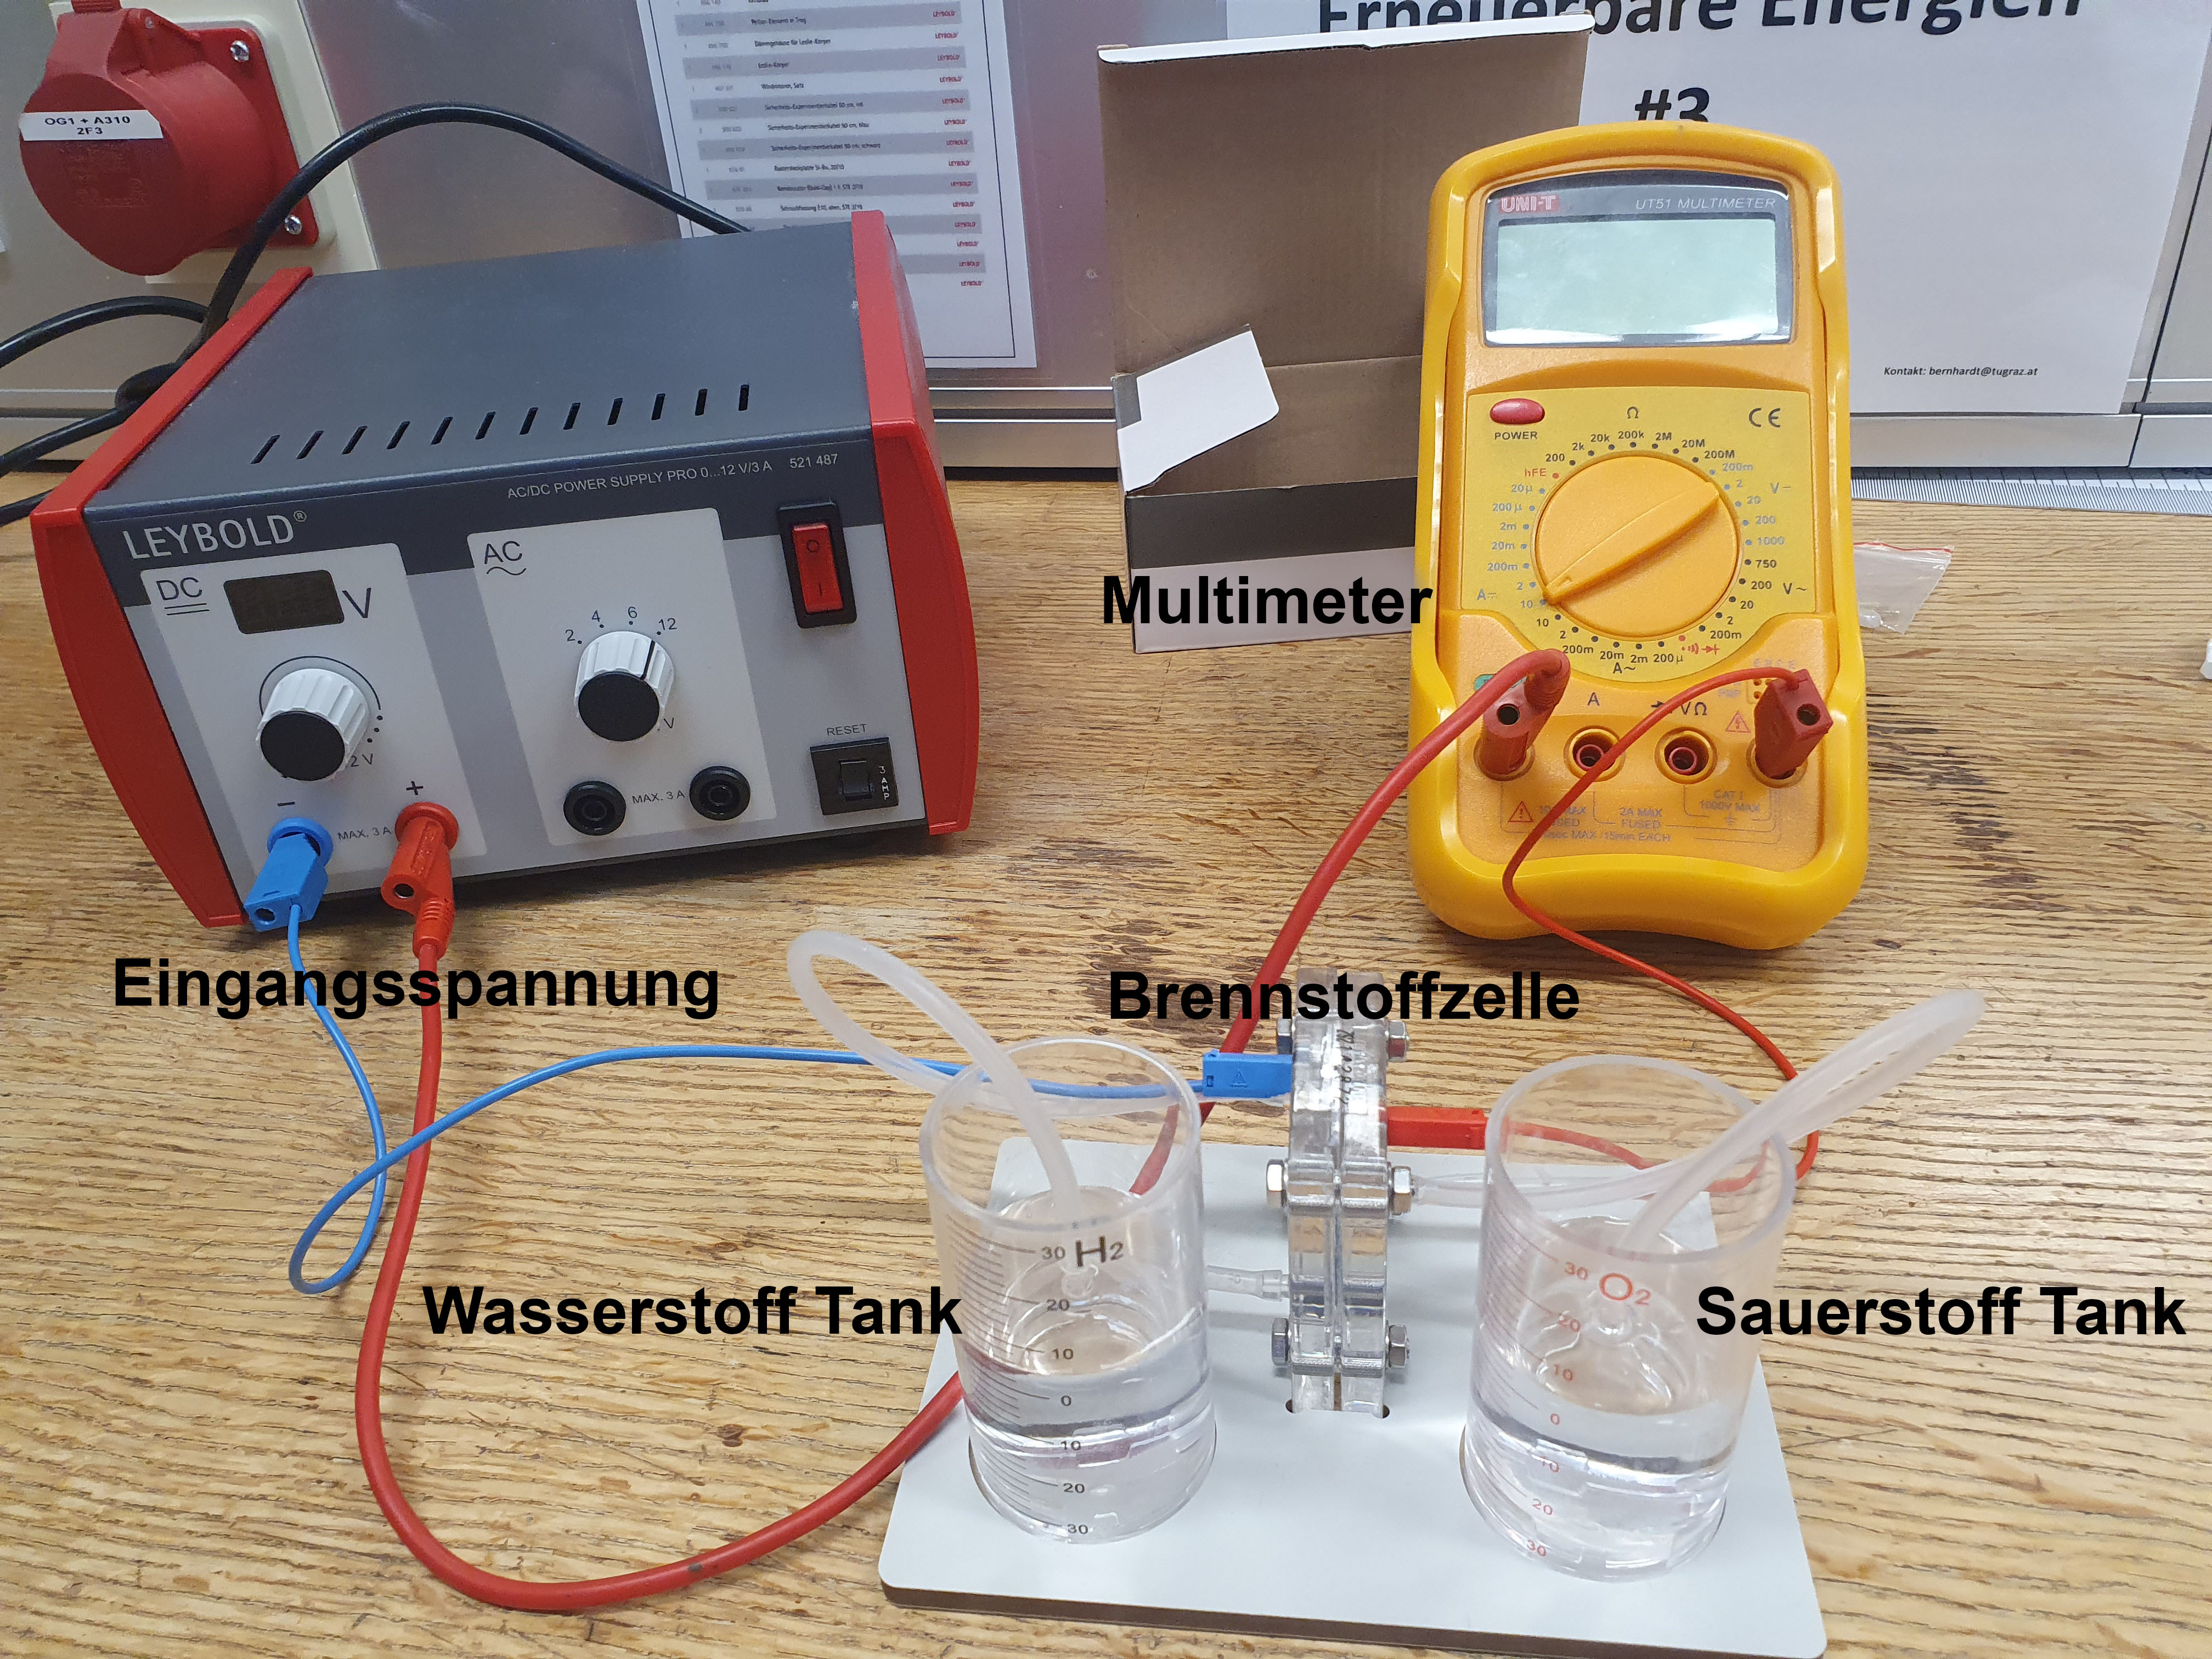
\includegraphics[width=0.6\linewidth]{nudes/brennstoff aufbau.jpg}
        \caption{Aufbau des Teilversuches Brennstoffzelle}
        \label{fig:aufbau Brennstoffzelle}
    \end{figure}

    \begin{figure}[H]
        \centering
        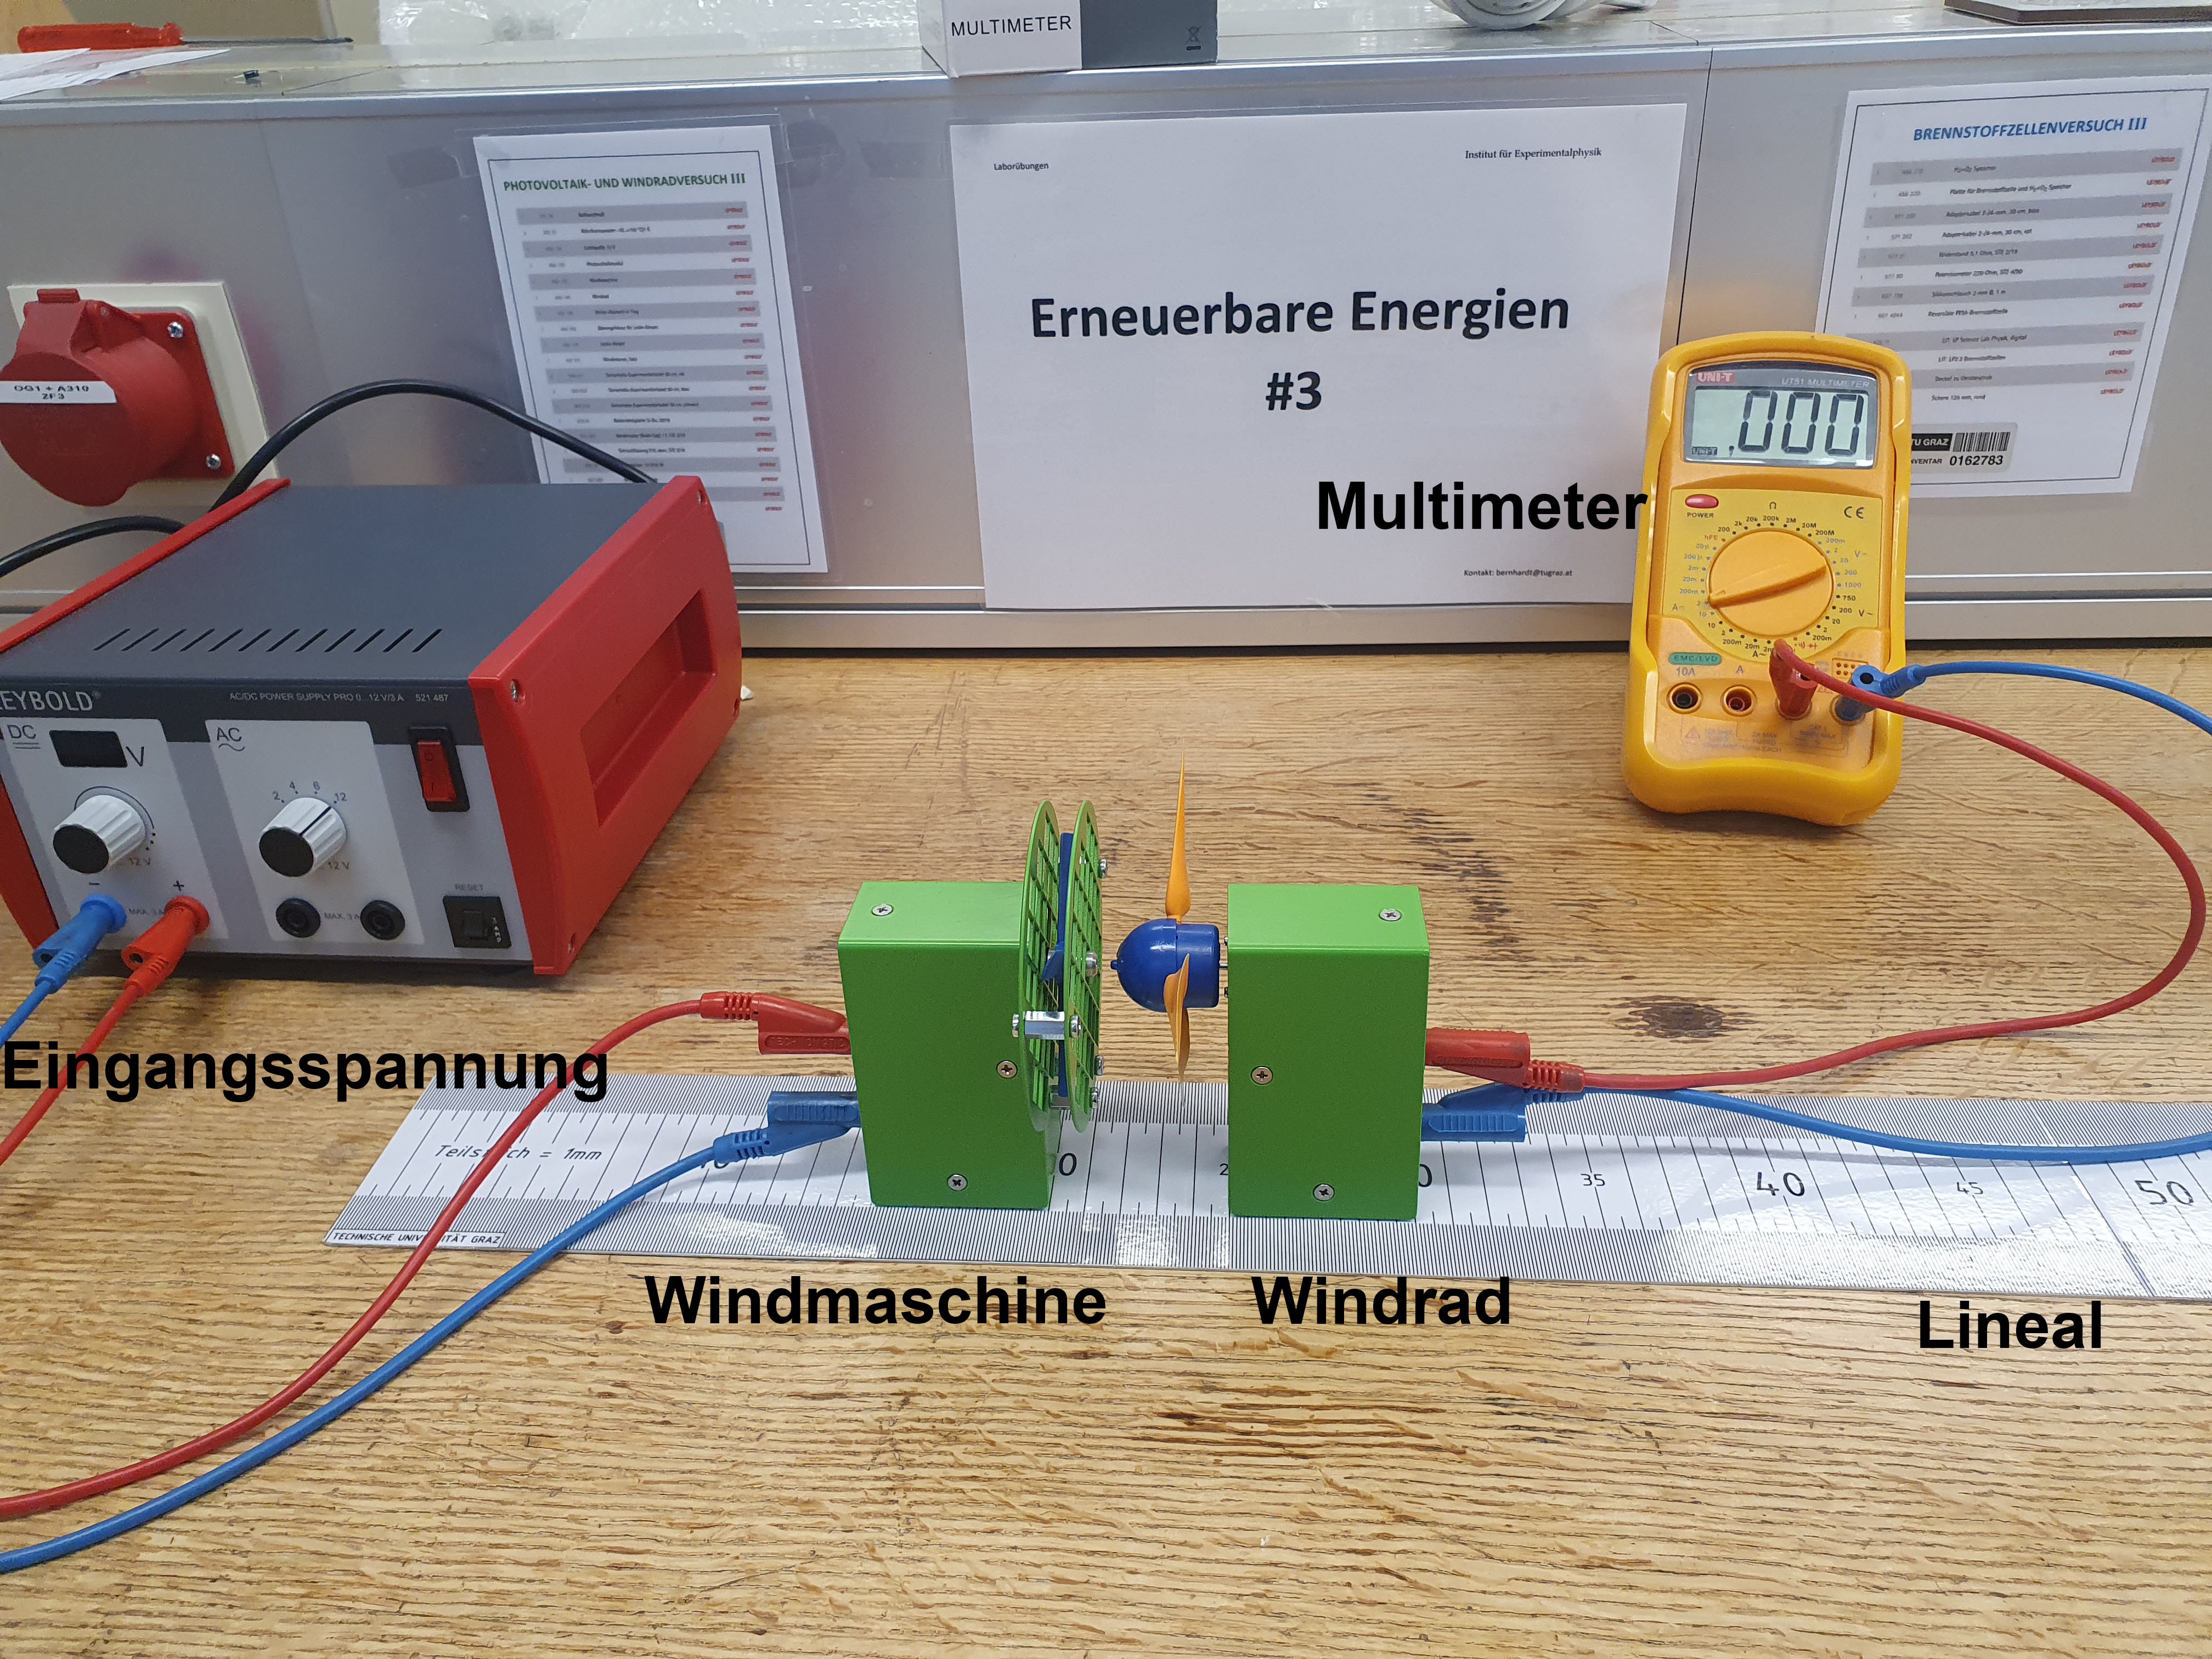
\includegraphics[width=0.6\linewidth]{nudes/wind aufbau.jpg}
        \caption{Aufbau des Teilversuches Windkraft}
        \label{fig:aufbau Windkraft}
    \end{figure}

    \begin{figure}[H]
        \centering
        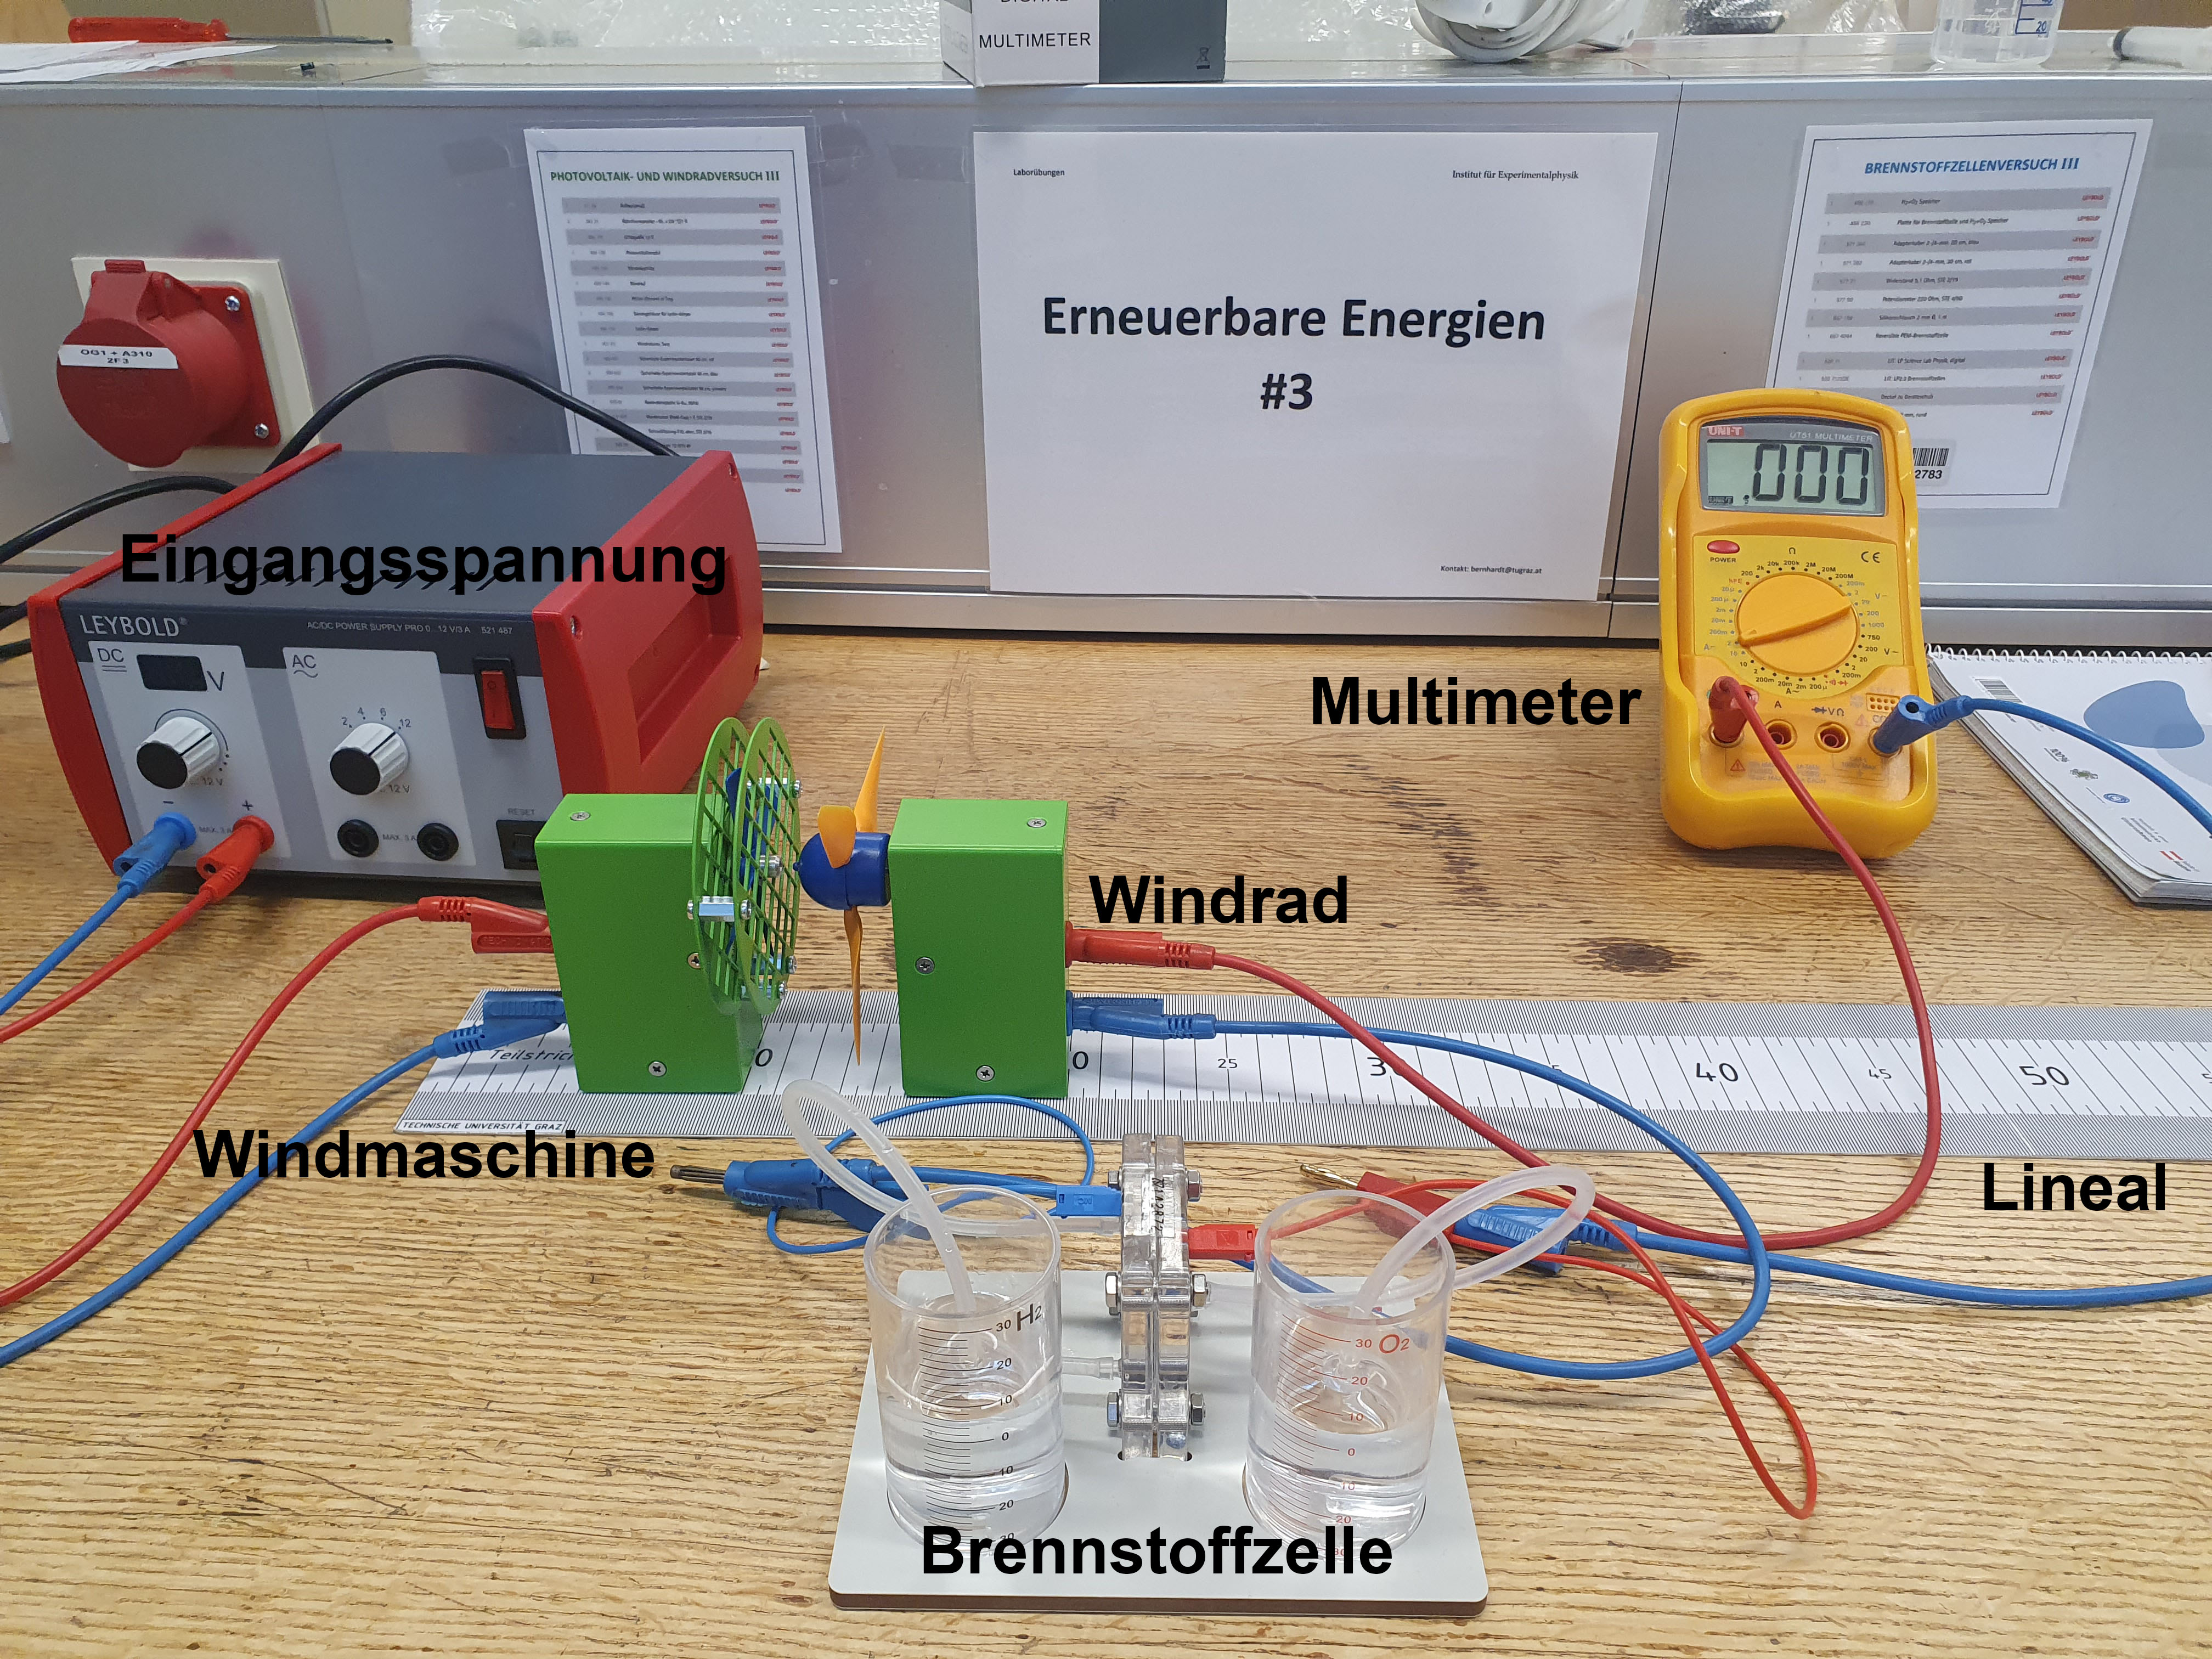
\includegraphics[width=0.6\linewidth]{nudes/wind und brennstoff.jpg}
        \caption{Aufbau des Teilversuches Speicherung der Energie}
        \label{fig:aufbau Speicherung Energie}
    \end{figure}

    \begin{figure}[H]
        \centering
        \includegraphics[width=0.6\linewidth]{nudes/schaltpläne.png}
        \caption{Zu vorbereitende Schaltpläne}
        \label{fig:schaltpläne}
    \end{figure}

\section{Geräteliste} %jo holt a listn ------------------------------

    \begin{table}[H]
        \centering
        \caption{Im Versuch verwendete Geräte und Utensilien.}
        \label{tab:geraete}
        \begin{tabular}{| l | l | l |}
            \hline
            Gerät  & Gerätenummer  & Unsicherheit \\
            \hline
            Leybold AC/DC PSU PRO 0...12 V/3 A& 521 487 & {n.a} \\
            Multimeter (Spannung) UNI-T & UT51 & $\pm (0.5 \% + 1 dig.)V$ \cite{multimeter1} \\
            Multimeter (Strom) UNI-T & UT51 & $\pm (0.8 \% + 1 dig.)A$  \cite{multimeter1} \\
            Multimeter Voltcraft & VC170-1 & $\pm (0.5 \% + 8 dig.)V$ \cite{multimeter2} \\
            Lineal & {n.a} & $\pm 1mm $ \\
            Stoppuhr Samsung S10+ & SM-G975F & $\pm 0.01s$ \\
            Kondensator & {n.a} & {n.a} \\
            Leuchte & {n.a} & {n.a} \\
            Solarzelle & {n.a} & {n.a} \\
            Brennstoffzelle & {n.a} & {n.a} \\
            Windmaschine & {n.a} & {n.a} \\
            Windrad & {n.a} & {n.a} \\
            Schaltboard & {n.a} & {n.a} \\
            \hline
        \end{tabular}
    \end{table}


\section{Versuchsdurchführung \& Messergebnisse} %nachvollziehbar und klar dargestellt ------------------------------

\subsection{Photovoltaik}
Im ersten Teilversuch wird die Schaltung laut Abbildung \ref{fig:aufbau Photovoltaik} aufgebaut. Der Abstand zwischen Lampe und Solarmodul beträgt $(30.0 \pm 0.1)cm $. 
Die Eingangsspannung beträgt 12V. 
Jeweils für die linke Solarzelle, die rechte Solarzelle, eine Parallelschaltung und eine Serienschaltung wird die Leerlaufspannung $U$ und der Kurzschlussstrom $I$ gemessen. 
\\
Aus den Messungen erhält man: 
\begin{itemize}
    \item $U_{Links} = (1.103 \pm 0.007)V$
    \item $U_{Rechts} = (1.098 \pm 0.007)V$
    \item $U_{Seriell} = (2.20 \pm 0.03)V$
    \item $U_{Parallel} = (1.10 \pm 0.02)V$
    
    \item $I_{Links} = (33.4 \pm 0.4)mA$
    \item $I_{Rechts} = (35.7 \pm 0.4)mA$
    \item $I_{Seriell} = (33.6 \pm 0.4)mA$
    \item $I_{Parallel} = (69.1 \pm 0.7)mA$
\end{itemize}

\noindent
Der Versuch ist für unterschiedliche Abstände $d$ der Lampe zum Solarmodul zu wiederholen. Die änderung des Abstandes erfolgt in 5cm Schritten. 

\begin{table}[H]
    \centering
    \caption{Leerlaufspannung $U$ des Solarmoduls bei verschiedenen Abständen $d$}
    \label{tab:Messdaten Spannung Solar}
    \begin{tabular}{| l | l | l | l | l | l |}
        \hline
        Nr. & $d \pm $ $0.1 $ / cm & $U_{L}$ / V & $U_{R}$ / V & $U_{Seriell}$ / V & $U_{Parallel}$ / V \\
        \hline
        1  & 5.0  & 1.149 $\pm$ 0.007 & 1.152 $\pm$ 0.007 & 2.30 $\pm$ 0.03 & 1.16 $\pm$ 0.02   \\
        2  & 10.0 & 1.142 $\pm$ 0.007 & 1.148 $\pm$ 0.007 & 2.30 $\pm$ 0.03 & 1.15 $\pm$ 0.02   \\
        3  & 15.0 & 1.109 $\pm$ 0.007 & 1.120 $\pm$ 0.007 & 2.24 $\pm$ 0.03 & 1.12 $\pm$ 0.02   \\
        4  & 20.0 & 1.082 $\pm$ 0.007 & 1.089 $\pm$ 0.007 & 2.18 $\pm$ 0.03 & 1.09 $\pm$ 0.02   \\
        5  & 25.0 & 1.060 $\pm$ 0.007 & 1.062 $\pm$ 0.007 & 2.13 $\pm$ 0.03 & 1.07 $\pm$ 0.02   \\
        6  & 30.0 & 1.042 $\pm$ 0.007 & 1.040 $\pm$ 0.007 & 2.09 $\pm$ 0.03 & 1.05 $\pm$ 0.02   \\
        7  & 35.0 & 1.028 $\pm$ 0.007 & 1.021 $\pm$ 0.007 & 2.06 $\pm$ 0.03 & 1.03 $\pm$ 0.02   \\
        8  & 40.0 & 1.014 $\pm$ 0.007 & 1.005 $\pm$ 0.007 & 2.02 $\pm$ 0.03 & 1.01 $\pm$ 0.02   \\
        9  & 45.0 & 1.004 $\pm$ 0.007 & 0.991 $\pm$ 0.006 & 2.00 $\pm$ 0.03 & 1.00 $\pm$ 0.02   \\
        10 & 50.0 & 0.995 $\pm$ 0.006 & 0.978 $\pm$ 0.006 & 1.97 $\pm$ 0.02 & 0.99 $\pm$ 0.02   \\
        11 & 55.0 & 0.987 $\pm$ 0.006 & 0.965 $\pm$ 0.006 & 1.95 $\pm$ 0.02 & 0.97 $\pm$ 0.02   \\
        12 & 60.0 & 0.980 $\pm$ 0.006 & 0.952 $\pm$ 0.006 & 1.93 $\pm$ 0.02 & 0.96 $\pm$ 0.02   \\
        13 & 65.0 & 0.974 $\pm$ 0.006 & 0.943 $\pm$ 0.006 & 1.91 $\pm$ 0.02 & 0.95 $\pm$ 0.02   \\
        14 & 70.0 & 0.968 $\pm$ 0.006 & 0.931 $\pm$ 0.006 & 1.89 $\pm$ 0.02 & 0.94 $\pm$ 0.02   \\
        15 & 75.0 & 0.963 $\pm$ 0.006 & 0.921 $\pm$ 0.006 & 1.87 $\pm$ 0.02 & 0.93 $\pm$ 0.02   \\
        16 & 80.0 & 0.953 $\pm$ 0.006 & 0.913 $\pm$ 0.006 & 1.86 $\pm$ 0.02 & 0.92 $\pm$ 0.02   \\
        17 & 85.0 & 0.944 $\pm$ 0.006 & 0.907 $\pm$ 0.006 & 1.84 $\pm$ 0.02 & 0.92 $\pm$ 0.02   \\
        18 & 90.0 & 0.938 $\pm$ 0.006 & 0.899 $\pm$ 0.006 & 1.82 $\pm$ 0.02 & 0.91 $\pm$ 0.02   \\
        \hline
    \end{tabular}
\end{table}

\begin{table}[H]
    \centering
    \caption{Kurzschlussstrom $I$ des Solarmoduls bei verschiedenen Abständen $d$}
    \label{tab:Messdaten Strom Solar}
    \begin{tabular}{| l | l | l | l | l | l |}
        \hline
        Nr. & $d \pm $ $0.1 $ / cm & $I_{L}$ / mA & $I_{R}$ / mA & $I_{Seriell}$ / mA & $I_{Parallel}$ / A \\
        \hline
        1  & 5.0  & 142.2 $\pm$ 1.3  & 79.6  $\pm$ 0.8 & 61.0  $\pm$ 0.6 & 0.265 $\pm$ 0.004  \\
        2  & 10.0 & 167.8 $\pm$ 1.5  & 155.1 $\pm$ 1.4 & 127.0 $\pm$ 1.1 & 0.261 $\pm$ 0.003  \\
        3  & 15.0 & 116.4 $\pm$ 1.1  & 111.8 $\pm$ 1.1 & 79.0  $\pm$ 0.8 & 0.202 $\pm$ 0.003  \\
        4  & 20.0 &  73.3 $\pm$ 0.7  & 71.8  $\pm$ 0.7 & 58.0  $\pm$ 0.5 & 0.136 $\pm$ 0.002  \\
        5  & 25.0 &  50.5 $\pm$ 0.5  & 50.2  $\pm$ 0.5 & 44.1  $\pm$ 0.4 & 0.096 $\pm$ 0.002  \\
        6  & 30.0 &  36.7 $\pm$ 0.4  & 37.1  $\pm$ 0.4 & 31.3  $\pm$ 0.4 & 0.071 $\pm$ 0.002  \\
        7  & 35.0 &  27.8 $\pm$ 0.4  & 28.3  $\pm$ 0.4 & 23.7  $\pm$ 0.4 & 0.054 $\pm$ 0.002  \\
        8  & 40.0 &  21.7 $\pm$ 0.3  & 22.1  $\pm$ 0.3 & 21.8  $\pm$ 0.3 & 0.043 $\pm$ 0.002  \\
        9  & 45.0 &  17.7 $\pm$ 0.3  & 17.7  $\pm$ 0.3 & 18.2  $\pm$ 0.3 & 0.034 $\pm$ 0.002  \\
        10 & 50.0 &  14.8 $\pm$ 0.3  & 15.0  $\pm$ 0.3 & 15.8  $\pm$ 0.3 & 0.028 $\pm$ 0.002  \\
        11 & 55.0 &  12.7 $\pm$ 0.2  & 13.6  $\pm$ 0.2 & 13.4  $\pm$ 0.2 & 0.024 $\pm$ 0.002  \\
        12 & 60.0 &  11.2 $\pm$ 0.2  & 11.7  $\pm$ 0.2 & 11.3  $\pm$ 0.2 & 0.021 $\pm$ 0.002  \\
        13 & 65.0 &  10.1 $\pm$ 0.2  & 10.1  $\pm$ 0.2 & 10.0  $\pm$ 0.2 & 0.018 $\pm$ 0.002  \\
        14 & 70.0 &   9.1 $\pm$ 0.2  & 9.0   $\pm$ 0.2 & 8.9   $\pm$ 0.2 & 0.016 $\pm$ 0.002  \\
        15 & 75.0 &   8.0 $\pm$ 0.2  & 8.1   $\pm$ 0.2 & 7.9   $\pm$ 0.2 & 0.015 $\pm$ 0.002  \\
        16 & 80.0 &   7.1 $\pm$ 0.2  & 7.4   $\pm$ 0.2 & 7.1   $\pm$ 0.2 & 0.013 $\pm$ 0.002  \\
        17 & 85.0 &   6.5 $\pm$ 0.2  & 6.7   $\pm$ 0.2 & 6.5   $\pm$ 0.2 & 0.013 $\pm$ 0.002  \\
        18 & 90.0 &   6.0 $\pm$ 0.2  & 6.1   $\pm$ 0.2 & 6.0   $\pm$ 0.2 & 0.012 $\pm$ 0.001  \\
        \hline  
    \end{tabular}
\end{table}

\subsection{Brennstoffzelle}
Bei dem Versuch mit der Brennstoffzelle wird die Schaltung wie in Abbildung \ref{fig:aufbau Brennstoffzelle} gezeigt aufgebaut. 
Die Brennstoffzelle wird mit Wasser befüllt. Die beiden Tanks werden bis zur 0-Linie mit Wasser gefüllt und die Gastanks werden eingesetzt und über Schläuche mit der Brennstoffzelle verbunden. 
Die Brennstoffzelle wird mit Spannung versorgt, es findet also eine kalte Verbrennung statt und Wasserstoff wird hergestellt. 
Die Eingangsspannung $U_{ein}$ wird langsam erhöht und der Strom $I_{gem}$ wird mit dem Multimeter gemessen. 
Dabei ist zu beobachten, ab welcher angelegten Spannung sich die Gastanks anfangen zu befüllen. Bei dem Versuch ist ein befüllen ab einer Eingangsspannung von $U_{ein} = (1.72 \pm 0.01) V$ beobachtbar gewesen. 
Ist das geschehen, so wird die Spannung erhöht, bis die Strömstärke 500 mA erreicht. 
\\
Die Unsicherheit der Spannung $U_{ein}$ ist die Ableseunsicherheit des Gerätes. 
\begin{table}[H]
    \centering
    \caption{Strom $I_{gem}$ in Abhängigkeit der Eingangsspannung $U_{ein}$ der Brennstoffzelle bei kalter Verbrennung. }
    \label{tab:Messdaten Brennstoffzelle}
    \begin{tabular}{| l | l | l |}
        \hline
        Nr. & $U_{ein} $ $\pm 0.01 $  / V & $I_{gem}$ / mA  \\
        \hline
        1  & 1.72  & 54  $\pm$ 2  \\
        2  & 1.80  & 84  $\pm$ 2  \\
        3  & 1.92  & 117 $\pm$ 2  \\
        4  & 2.00  & 144 $\pm$ 3  \\
        5  & 2.12  & 171 $\pm$ 3  \\
        6  & 2.24  & 214 $\pm$ 3  \\
        7  & 2.32  & 225 $\pm$ 3  \\
        8  & 2.44  & 259 $\pm$ 4  \\
        9  & 2.52  & 284 $\pm$ 4  \\
        10 & 2.64  & 315 $\pm$ 4  \\
        11 & 2.72  & 339 $\pm$ 4  \\
        12 & 2.80  & 369 $\pm$ 4  \\
        13 & 2.92  & 418 $\pm$ 5  \\
        14 & 3.00  & 444 $\pm$ 5  \\
        15 & 3.12  & 495 $\pm$ 5  \\
        \hline  
    \end{tabular}
\end{table}

\noindent
Die Gastanks sind vom vorherigen Teil mit Wasserstoff und Sauerstoff gefüllt. Das Volumen beträgt dabei in beiden Tanks $(20 \pm 1) ml$ (Unsicherheit implizit angenommen).  
In die Schaltung wird ein Potentiometer (Stellung g), sowie ein Widerstand mit $(5.1 \pm 0.1) \Omega$ eingefügt (Unsicherheit implizit angenommen). 
Durch Messung der Volumensänderung im Wasserstofftank pro Zeit, sowie Strom und Spannung, lässt sich die Leistung berechnen, sowie die geleistete Arbeit. 
\\
Das Volumen im Wasserstofftank verringert sich auf $(12 \pm 1)$ ml in einer Zeit von $(289.4 \pm 0.1) s $ (Unsicherheit der Handystoppuhr implizit angenommen). 
Die Spannung $U$ beträgt dabei $(0.74 \pm 0.09)V$ und der Strom $I$ beträgt $(0.14 \pm 0.02)A$. 
\\
\\
Um die Kennlinie der Brennstoffzelle zu bestimmen, bleibt der Aufbau wie im vorherigen Punkt. 
Ohne zusätzlichen Widerstand wird der Widerstand am Potentiometer schrittweise verringert. Dabei wird die Spannung $U$ und der Strom $I$ aufgezeichnet. 
Durch hinzufügen eines Widerstandes von $(5.1 \pm 0.1) \Omega$ parallel zum Potentiometer wird der Versuch erneut durchgeführt. 

\begin{table}[H]
    \centering
    \caption{Messdaten der Spannung $U$ und des Stromes $I$ zur bestimmung der Kennlinie}
    \label{tab:Messdaten Kennlinie Brennstoffzelle}
    \begin{tabular}{| l | l | l | l | l | l |}
        \hline
        Nr. & Potentiometer & $U_{ohneR}$  / V & $I_{ohneR}$ / A & $U_{mitR}$ / V & $I_{mitR}$ / A \\
        \hline
        1  & g    & 0     $\pm$ 0.008 & 0.949 $\pm$ 0.009 & 0.14 $\pm$ 0.009 & 0.720 $\pm$ 0.007 \\
        2  & g-f  & 0     $\pm$ 0.008 & 0.947 $\pm$ 0.009 & 0.13 $\pm$ 0.009 & 0.635 $\pm$ 0.007 \\
        3  & f    & 0.001 $\pm$ 0.009 & 0.944 $\pm$ 0.009 & 0.12 $\pm$ 0.009 & 0.590 $\pm$ 0.006 \\
        4  & f-e  & 0.001 $\pm$ 0.009 & 0.938 $\pm$ 0.009 & 0.11 $\pm$ 0.009 & 0.540 $\pm$ 0.006 \\
        5  & e    & 0.001 $\pm$ 0.009 & 0.934 $\pm$ 0.009 & 0.10 $\pm$ 0.009 & 0.481 $\pm$ 0.005 \\
        6  & e-d  & 0.001 $\pm$ 0.009 & 0.928 $\pm$ 0.009 & 0.09 $\pm$ 0.009 & 0.414 $\pm$ 0.005 \\
        7  & d    & 0.001 $\pm$ 0.009 & 0.923 $\pm$ 0.009 & 0.08 $\pm$ 0.009 & 0.400 $\pm$ 0.005 \\
        8  & d-c  & 0.001 $\pm$ 0.009 & 0.916 $\pm$ 0.009 & 0.08 $\pm$ 0.009 & 0.381 $\pm$ 0.005 \\
        9  & c    & 0.001 $\pm$ 0.009 & 0.905 $\pm$ 0.009 & 0.07 $\pm$ 0.009 & 0.352 $\pm$ 0.004 \\
        10 & c-b  & 0.002 $\pm$ 0.009 & 0.892 $\pm$ 0.009 & 0.07 $\pm$ 0.009 & 0.304 $\pm$ 0.004 \\
        11 & b    & 0.003 $\pm$ 0.009 & 0.875 $\pm$ 0.008 & 0.06 $\pm$ 0.009 & 0.276 $\pm$ 0.004 \\
        12 & b-a  & 0.008 $\pm$ 0.009 & 0.818 $\pm$ 0.008 & 0.06 $\pm$ 0.009 & 0.215 $\pm$ 0.003 \\
        13 & a    & 0.030 $\pm$ 0.009 & 0.250 $\pm$ 0.003 & 0.06 $\pm$ 0.009 & 0.040 $\pm$ 0.002 \\
        \hline  
    \end{tabular}
\end{table}

\subsection{Windkraft}
Der Versuch wird wie in Abbildung \ref{fig:aufbau Windkraft} aufgebaut. Der Abstand zwischen Windmaschine und Windrad beträgt $(5.0 \pm 0.1)cm$. 
Die Eingangsspannung $U_{ein}$ wird langsam erhöht, und die Leerlaufspannung $U_{leer}$ am Windrad wird gemessen. 

\begin{table}[H]
    \centering
    \caption{Leerlaufspannung des Windrades}
    \label{tab:Messdaten Windkraft stationär}
    \begin{tabular}{| l | l | l |}
        \hline
        Nr. & $U_{ein} $ $\pm$ 0.01 / V & $U_{leer}$ / V \\
        \hline
        1  & 5.28  & 3.12 $\pm$ 0.03  \\
        2  & 5.79  & 3.50 $\pm$ 0.03  \\
        3  & 6.12  & 3.77 $\pm$ 0.03    \\
        4  & 6.76  & 4.22 $\pm$ 0.04   \\
        5  & 7.20  & 4.51 $\pm$ 0.04    \\
        6  & 7.68  & 4.82 $\pm$ 0.04   \\
        7  & 8.12  & 5.13 $\pm$ 0.04    \\
        8  & 8.76  & 5.57 $\pm$ 0.04    \\
        9  & 9.30  & 5.94 $\pm$ 0.04   \\
        10 & 9.69  & 6.19 $\pm$ 0.04    \\
        \hline  
    \end{tabular}
\end{table}

\noindent
Im zweiten Teil wird die Eingangsspannung $U_{ein}$ auf $(10 \pm 0.01)V$ fixiert und der Abstand $d$ zwischen Windmaschine und Windrad wird schrittweise erhöht. 
Die Leerlaufspannung $U_{leer}$ wird gemessen. 
\begin{table}[H]
    \centering
    \caption{Leerlaufspannung $U_{leer}$ bei unterschiedlichen Abständen $d$ zur Windmaschine}
    \label{tab:Messdaten Windkraft mit d}
    \begin{tabular}{| l | l | l | l |}
        \hline
        Nr. & $U_{ein} $ $\pm $ 0.01 / V & $U_{leer}$ / V & d $\pm$ 0.1 / cm \\
        \hline
        1  & 10.0  & 6.45 $\pm$ 0.05  & 5 \\
        2  & 10.0  & 6.07 $\pm$ 0.04  & 7 \\
        3  & 10.0  & 5.64 $\pm$ 0.04  & 9 \\
        4  & 10.0  & 4.76 $\pm$ 0.04  & 11 \\
        5  & 10.0  & 4.40 $\pm$ 0.04  & 13 \\
        6  & 10.0  & 4.25 $\pm$ 0.04  & 15 \\
        7  & 10.0  & 3.67 $\pm$ 0.03  & 17 \\
        8  & 10.0  & 2.91 $\pm$ 0.03  & 19 \\
        9  & 10.0  & 2.42 $\pm$ 0.03  & 21 \\
        10 & 10.0  & 2.05 $\pm$ 0.02  & 23 \\
        \hline  
    \end{tabular}
\end{table}

\noindent
In diesen Teil werden mehrere Szenarien getestet. Dabei wird die Energie, welche das Windrad erzeugt in Form von einem elektrischen Potential gespeichert.
Die Schaltung wird wie bei Teil 1 laut Abbildung \ref{fig:aufbau Windkraft} aufgebaut. Der Abstand $d$ wird dabei auf $(15 \pm 0.1)cm$ festgelegt. 
Durch den gewählten Abstand beträgt die Maximale Spannung $(4.52 \pm 0.04)V$. 
\\
Im ersten Szenario wird getestet, wie sich die Spannung $U$ verhält, wenn der Luftstrom abrupt gestoppt wird. 
Dabei wird die Zeit $t$ jede Sekunde nach dem Abschalten, sowie die Spannung $U$ gemessen. 

\begin{table}[H]
    \centering
    \caption{Spannung $U$ pro Sekunde nach abbrupten Abschalten}
    \label{tab:Messdaten Windkraft abbrupt stop}
    \begin{tabular}{| l | l | l |}
        \hline
        Nr. & $t$ $\pm $ 0.1 / s & $U$ / V \\
        \hline
        1  & 0  & 4.52 $\pm$ 0.04   \\
        2  & 1  & 3.53 $\pm$ 0.03   \\
        3  & 2  & 2.37 $\pm$ 0.03   \\
        4  & 3  & 1.87 $\pm$ 0.02   \\
        5  & 4  & 1.50 $\pm$ 0.02   \\
        6  & 5  & 1.21 $\pm$ 0.02   \\
        7  & 6  & 0.98 $\pm$ 0.02   \\
        8  & 7  & 0.69 $\pm$ 0.02   \\
        9  & 8  & 0.54 $\pm$ 0.02   \\
        10 & 9  & 0.32 $\pm$ 0.02  \\
        11 & 10 & 0.19 $\pm$ 0.02   \\
        12 & 11 & 0.00 $\pm$ 0.01   \\
        \hline  
    \end{tabular}
\end{table}

\noindent
Das zweite Szenario testet, was passiert, wenn der Luftstrom abbrupt startet. 
\begin{table}[H]
    \centering
    \caption{Spannung $U$ pro Sekunde nach abbrupten Start}
    \label{tab:Messdaten Windkraft abbrupt start}
    \begin{tabular}{| l | l | l |}
        \hline
        Nr. & $t$ $\pm $ 0.1 / s & $U$ / V \\
        \hline
        1  & 0  & 0.00 $\pm$ 0.01   \\
        2  & 1  & 0.03 $\pm$ 0.02   \\
        3  & 2  & 0.26 $\pm$ 0.02   \\
        4  & 3  & 0.56 $\pm$ 0.02   \\
        5  & 4  & 0.88 $\pm$ 0.02   \\
        6  & 5  & 1.26 $\pm$ 0.02   \\
        7  & 6  & 2.02 $\pm$ 0.02   \\
        8  & 7  & 2.83 $\pm$ 0.03   \\
        9  & 8  & 3.50 $\pm$ 0.03   \\
        10 & 9  & 4.10 $\pm$ 0.04   \\
        11 & 10 & 4.36 $\pm$ 0.04   \\
        12 & 11 & 4.52 $\pm$ 0.04   \\
        \hline  
    \end{tabular}
\end{table}

\noindent
Im dritten Szenario werden die beiden vorherigen Szenarios erneut getestet, nur mit einem Kondensator zwischen Windrad und Multimeter. 
Hierbei wird die Spannung $U$ alle 5 Sekunden gemessen. 

\begin{table}[H]
    \centering
    \caption{Spannung $U$ nach abbrupten Stop und Start mit Kondensator}
    \label{tab:Messdaten Windkraft abbrupt stop kondensator}
    \begin{tabular}{| l | l | l | l |}
        \hline
        Nr. & $t$ $\pm $ 0.1 / s & $U_{Stop}$ / V & $U_{Start}$ / V \\
        \hline
        1  & 0  & 3.05 $\pm$ 0.03  & 0.00 $\pm$ 0.01  \\
        2  & 5  & 1.79 $\pm$ 0.02  & 0.45 $\pm$ 0.02  \\
        3  & 10 & 1.48 $\pm$ 0.02  & 1.11 $\pm$ 0.02  \\
        4  & 15 & 1.33 $\pm$ 0.02  & 1.92 $\pm$ 0.02  \\
        5  & 20 & 1.21 $\pm$ 0.02  & 2.44 $\pm$ 0.03  \\
        6  & 25 & 1.12 $\pm$ 0.02  & 2.78 $\pm$ 0.03  \\
        7  & 30 & 1.03 $\pm$ 0.02  & 2.98 $\pm$ 0.03  \\
        8  & 35 & 0.95 $\pm$ 0.02  & 3.16 $\pm$ 0.03  \\
        9  & 40 & 0.87 $\pm$ 0.02  & 3.32 $\pm$ 0.03  \\
        10 & 45 & 0.80 $\pm$ 0.02  & 3.48 $\pm$ 0.03  \\
        11 & 50 & 0.72 $\pm$ 0.02  & 3.58 $\pm$ 0.03  \\
        12 & 55 & 0.65 $\pm$ 0.02  &   \\
        13 & 60 & 0.58 $\pm$ 0.02  &   \\
        \hline  
    \end{tabular}
\end{table}

\noindent
Im letzten Teil wird die erzeugte Spannung des Windrades als Spannungsquelle für die Brennstoffzelle verwendet. 
Die Schaltung wird wie in Abbildung \ref{fig:aufbau Speicherung Energie} aufgebaut. 
Die Eingangsspannung $U_{ein}$ beträgt $(10.0 \pm 0.1)V$, der Abstand $d = (5 \pm 0.1)cm$ beträgt . Bei Start der Messung betrug der Stand im Wasserstofftank $(8 \pm 1)ml$ und im Sauerstofftank $(5 \pm 1)ml$
Beim Stoppen der Messung betrug der Stand im Wasserstofftank $(12 \pm 1)ml$ und im Sauerstofftank $(7 \pm 1)ml$. Dies dauerte insgesamt $(267.5 \pm 0.1) s$. 


\section{Auswertung und Unsicherheitsanalyse} %Nicht nur zahlen angeben ------------------------------

In der Auswertung werden zur erhöhten Genauigkeit durchgehend ungerundete Werte bis zu den Endergebnissen verwendet und nur zur Darstellung gerundet. \\
Zur Berechnung der Unsicherheiten wird, wenn nicht anders angegeben, die Größtunsicherheitsmethode verwendet.

\subsection{Photovoltaik}
Wie man aus der Aufzählung der Messergebnisse in Sektion Photovoltaik der Versuchsdurchführung erkennen kann, 
addieren sich die Spannungen $U$, wenn man die beiden Solarmodule in Serie schaltet. Bei der Strommessung lässt sich erkennen, dass bei Parallelschaltung der Strom $I$ der einzelnen Module addiert wird. 
\\
\\
Die Spannungen $U$ und Ströme $I$ der Abstandsmessungen werden in den nachfolgenden Diagrammen dargestellt. 

\begin{figure}[H]
    \centering
    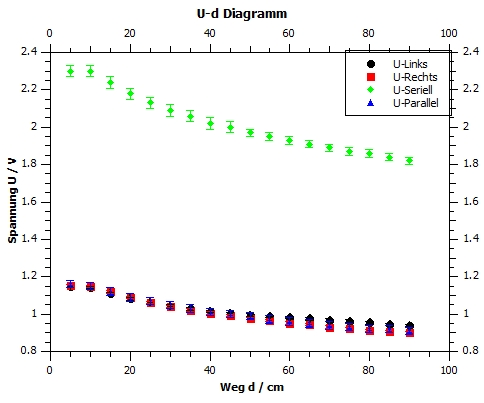
\includegraphics[width=0.6\linewidth]{nudes/u-d diagramm.jpg}
    \caption{Spannungen $U$ der einzelnen Schaltungen des Solarmoduls bei verschiedenen Abständen $d$}
    \label{fig:diagramm Photovoltaik U-d}
\end{figure}

\begin{figure}[H]
    \centering
    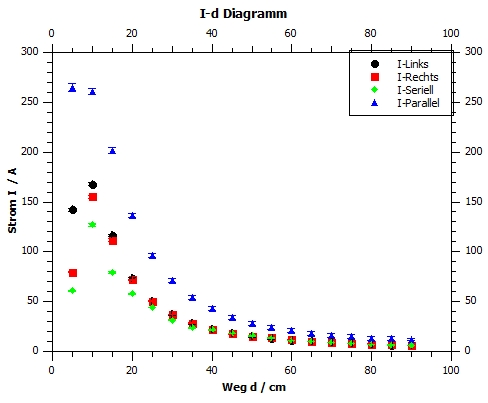
\includegraphics[width=0.6\linewidth]{nudes/i-d diagramm.jpg}
    \caption{Ströme $I$ der einzelnen Schaltungen des Solarmoduls bei verschiedenen Abständen $d$}
    \label{fig:diagramm Photovoltaik I-d}
\end{figure}

\noindent
Bei den Diagramm der Spannung $U$ lässt sich erkennen, dass die Spannung $U$ linear abfällt mit dem Abstand $d$ zur Lichtquelle. Bei der Seriellschaltung (grün) erkennt man, dass die einzelnen Spannungen $U_{Links}$ (schwarz) und $U_{Rechts}$ (rot) addiert werden, die Parallelschaltung (blau) hingegen wird nicht addiert. 
Im gegenzug bei dem Diagramm der Stromstärke $I$ erkennt man einen exponentiellen Abfall der Stromstärke $I$. Bei der Parallelschaltung (blau) erkennt man, dass die einzelnen Ströme $I_{Links}$ (schwarz) und $I_{Rechts}$ (rot) addiert werden. 

\subsection{Brennstoffzelle}
Die Daten aus der Tabelle \ref{tab:Messdaten Brennstoffzelle} werden als Diagramm dargestellt. Dabei ist anzumerken, dass die Gastanks sich ab einer Spannung von $U = (1.72 \pm 0.01)V$ zu füllen beginnen. 
Die Brennstoffzelle wandelt in diesen Versuch elektrische Energie in chemische Energie um. Es findet daher eine kalte Verbrennung statt. 

\begin{figure}[H]
    \centering
    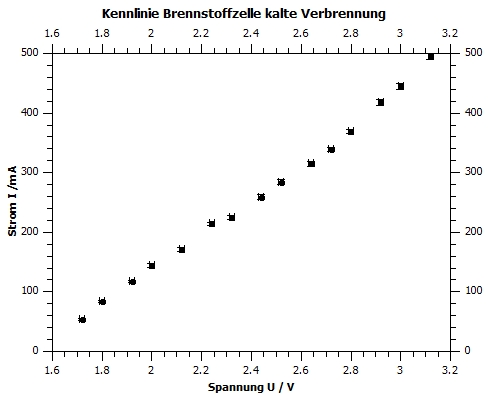
\includegraphics[width=0.6\linewidth]{nudes/brennstoff diagramm i-u.jpg}
    \caption{Kennlinie der Brennstoffzelle bei kalter Verbrennung. Der Strom $I$ in Abhängigkeit der Eingangsspannung $U$}
    \label{fig:diagramm Brennstoffzelle I-U}
\end{figure}

\noindent
Im zweiten Teil gilt es die Leistung der Brennstoffzelle zu berrechnen. Dazu benötigt man die Spannung $U$ und den Strom $I$. 
Eingesetzt in die Formel \ref{eq:leistung} kann man die Leistung $P$ berrechnen und kommt auf einen Wert von $P = (0.10 \pm 0.02)W$. 
\\
Die Energie $E$ lässt sich aus der Leistung $P$ und der Zeit $t$ pro Volumeneinheit berrechnen. Die Zeit $t$ pro Volumeneinheit lässt sich mit dem Kehrwert Formel \ref{eq:prominute} berrechnen und man erhält für die Zeit $t = (0.63 \pm 0.09)min$, was in Sekunden $t = (36.2 \pm 5.4)s$ entspricht. 
Mit diesen Werten und der Formel \ref{eq:energie} kommt man für die Energie $E$ auf den Wert von $E = (3.7 \pm 1.3)J$. 
Um den Wirkungsgrad zu berrechnen benötigt man die Leistung $P$, sowie die zugeführte Energie $E_{zu}$. Diese lässt sich aus der Energie $E$ sowie der Molzahl des verbrauchten Wasserstoffes berrechnen. Eine Volumeneinheit beträgt dabei 1ml, was 0.09g entspricht. 
Eingesetzt in die Formel \ref{eq:wirkungsgrad} mit einer Molaren Masse des Wasserstoff von 2.016 g/mol, erhält man einen Wirkungsgrad von $\eta = (60.6 \pm 40.1)\%$. 
\\
\\
Im dritten Teil wird für die Werte aus der Tabelle \ref{tab:Messdaten Kennlinie Brennstoffzelle} die Spannung $U$ in Abhängigkeit des Stromes $I$ dargestellt. 

\begin{figure}[H]
    \centering
    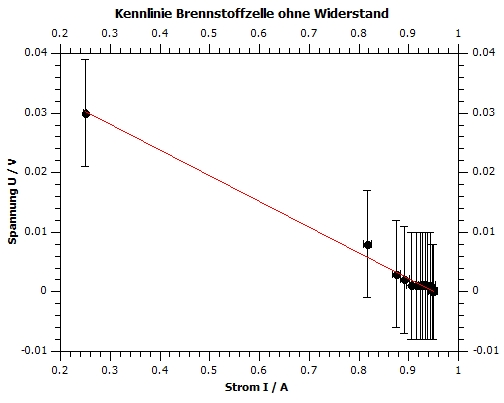
\includegraphics[width=0.6\linewidth]{nudes/brennstoff diagramm ohne r.jpg}
    \caption{Kennlinie der Brennstoffzelle bei Elektrolyse ohne Widerstand $R$. Die Spannung $U$ in Abhängigkeit des Stromes $I$. Mit der Steigung (rote Linie) von $(-0.043 \pm 0.014)$}
    \label{fig:diagramm Brennstoffzelle ohne R}
\end{figure}

\begin{figure}[H]
    \centering
    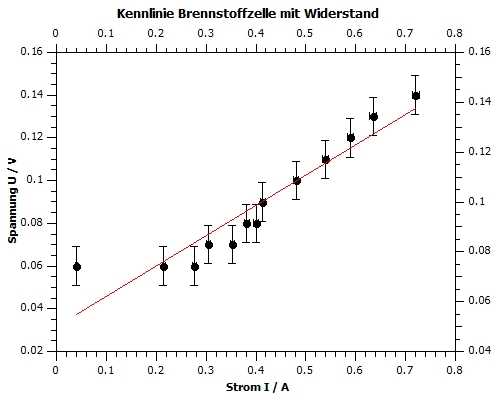
\includegraphics[width=0.6\linewidth]{nudes/brennstoff diagramm mit r.jpg}
    \caption{Kennlinie der Brennstoffzelle bei Elektrolyse mit Widerstand $R$. Die Spannung $U$ in Abhängigkeit des Stromes $I$. Mit der Steigung (rote Linie) von $(0.142 \pm 0.014)$}
    \label{fig:diagramm Brennstoffzelle mit R}
\end{figure}

\noindent
Desweiteren wird die Leistung $P$, welche mit der Formel \ref{eq:leistung} berechnet wird in einen Diagramm in Abhängigkeit des Stromes $I$ dargestellt und quadratisch genähert. 

\begin{table}[H]
    \centering
    \caption{Leistung $P$ der Brennstoffzelle in Abhängigkeit des Stromes $I$}
    \label{tab:Leistung Brennstoffzelle}
    \begin{tabular}{| l | l | l | l | l |}
        \hline
        Nr. & $P_{ohneR}$  / W & $I_{ohneR}$ / A & $P_{mitR}$ / W & $I_{mitR}$ / A \\
        \hline
        1   & 0       $\pm$ 0.008  & 0.949 $\pm$ 0.009 & 0.109   $\pm$ 0.008  & 0.720 $\pm$ 0.007 \\
        2   & 0       $\pm$ 0.008  & 0.947 $\pm$ 0.009 & 0.087   $\pm$ 0.007  & 0.635 $\pm$ 0.007 \\
        3   & 0.001   $\pm$ 0.009  & 0.944 $\pm$ 0.009 & 0.079   $\pm$ 0.007  & 0.590 $\pm$ 0.006 \\
        4   & 0.001   $\pm$ 0.009  & 0.938 $\pm$ 0.009 & 0.060   $\pm$ 0.006  & 0.540 $\pm$ 0.006 \\
        5   & 0.001   $\pm$ 0.009  & 0.934 $\pm$ 0.009 & 0.049   $\pm$ 0.005  & 0.481 $\pm$ 0.005 \\
        6   & 0.001   $\pm$ 0.009  & 0.928 $\pm$ 0.009 & 0.038   $\pm$ 0.005  & 0.414 $\pm$ 0.005 \\
        7   & 0.001   $\pm$ 0.009  & 0.923 $\pm$ 0.009 & 0.033   $\pm$ 0.004  & 0.400 $\pm$ 0.005 \\
        8   & 0.001   $\pm$ 0.009  & 0.916 $\pm$ 0.009 & 0.031   $\pm$ 0.004  & 0.381 $\pm$ 0.005 \\
        9   & 0.001   $\pm$ 0.009  & 0.905 $\pm$ 0.009 & 0.025   $\pm$ 0.004  & 0.352 $\pm$ 0.004 \\
        10  & 0.002   $\pm$ 0.009  & 0.892 $\pm$ 0.009 & 0.022   $\pm$ 0.004  & 0.304 $\pm$ 0.004 \\
        11  & 0.003   $\pm$ 0.008  & 0.875 $\pm$ 0.008 & 0.017   $\pm$ 0.003  & 0.276 $\pm$ 0.004 \\
        12  & 0.007   $\pm$ 0.008  & 0.818 $\pm$ 0.008 & 0.013   $\pm$ 0.003  & 0.215 $\pm$ 0.003 \\
        13  & 0.008   $\pm$ 0.003  & 0.250 $\pm$ 0.003 & 0.003   $\pm$ 0.001  & 0.040 $\pm$ 0.002 \\
        \hline  
    \end{tabular}
\end{table}

\begin{figure}[H]
    \centering
    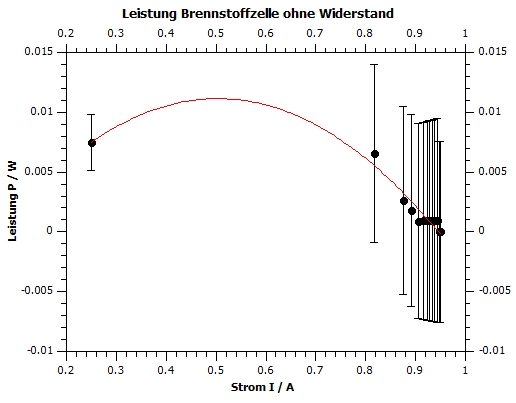
\includegraphics[width=0.6\linewidth]{nudes/brennstoff leistung ohne r.jpg}
    \caption{Leistung $P$ der Brennstoffzelle bei Elektrolyse ohne Widerstand $R$. Die Leistung $P$ wird in Abhängigkeit des Stromes $I$ dargestellt und quadratisch genähert (rote Kurve).}
    \label{fig:diagramm Leistung ohne R}
\end{figure}

\begin{figure}[H]
    \centering
    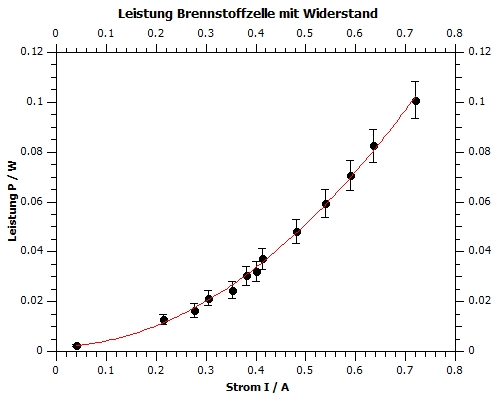
\includegraphics[width=0.6\linewidth]{nudes/brennstoff leistung mit r.jpg}
    \caption{Leistung $P$ der Brennstoffzelle bei Elektrolyse mit Widerstand $R$. Die Leistung $P$ wird in Abhängigkeit des Stromes $I$ dargestellt und quadratisch genähert (rote Kurve).}
    \label{fig:diagramm Leistung mit R}
\end{figure}

\subsection{Windkraft}
Bei dem Versuch Windkraft wird im ersten Teil die Eingangsspannung $U_{ein}$ erhöht. Die Leerlaufspannung $U_{leer}$ steigt linear dazu an. Sieht man sich das folgende Diagramm an, welches die Leerlaufspannung $U_{leer}$ in relation zur Eingangsspannung $U_{ein}$ aus den Daten der Tabelle \ref{tab:Messdaten Windkraft stationär} zeigt, 
erkennt man einen linearen Anstieg. 

\begin{figure}[H]
    \centering
    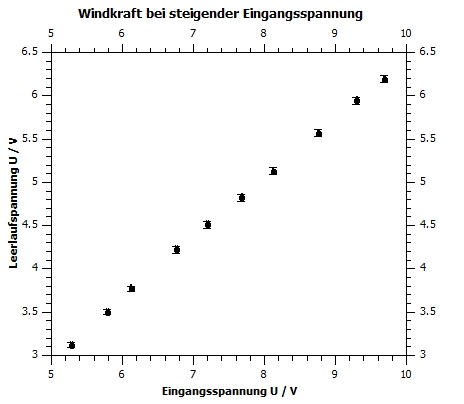
\includegraphics[width=0.6\linewidth]{nudes/wind spannung.jpg}
    \caption{Spannungen U der Windkraft bei fixem Abstand $d$ von 5cm}
    \label{fig:windkraft stationär diagramm}
\end{figure}

\noindent
Hingegen bei fixer Eingangsspannung $U_{ein}$ von $(10.0 \pm 0.1)V$ und steigenden Abstand $d$ sinkt die Leerlaufspannung $U_{leer}$ linear. 
Aus den Messdaten der Tabelle \ref{tab:Messdaten Windkraft mit d} wird das Diagramm bebildet, was einen linearen Abfall der Leerlaufspannung $U_{leer}$ mit zunehmenden Abstand $d$ zeigt. 

\begin{figure}[H]
    \centering
    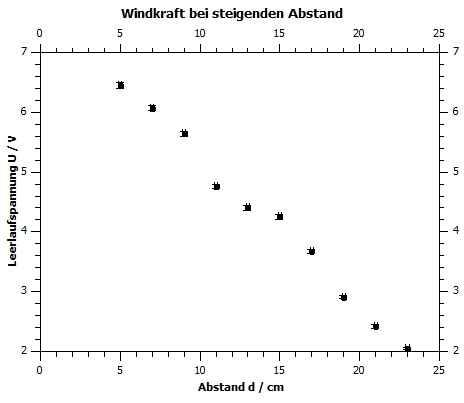
\includegraphics[width=0.6\linewidth]{nudes/wind abstand.jpg}
    \caption{Leerlaufspannung $U_{leer}$ der Windkraft bei fixer Eingangsspannung $U_{ein}$ und steigenden Abstand $d$}
    \label{fig:windkraft abstand diagramm}
\end{figure}

\noindent
Bricht man den Luftstrom abbrupt ab, so fällt die Leerlaufspannung $U_{leer}$ anfangs schneller ab, als nach einer gewissen Zeit $t$, da das Windrad noch ein gewisses Drehmoment besitzt. 
Mit den Messdaten der Tabelle \ref{tab:Messdaten Windkraft abbrupt stop} wird ein Diagramm geplottet, in welchem man den Verlauf der Leerlaufspannung $U_{leer}$ pro Zeit $t$ sieht. 

\begin{figure}[H]
    \centering
    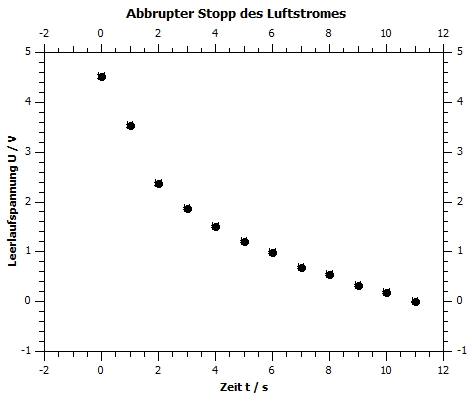
\includegraphics[width=0.6\linewidth]{nudes/wind stopp.jpg}
    \caption{Leerlaufspannung $U_{leer}$ der Windkraft bei abbrupten Stopp des Luftstromes pro Sekunde.}
    \label{fig:windkraft stopp diagramm}
\end{figure}

\noindent
Hingegen startet man den Luftstrom abbrupt, so lässt sich ein erst langsamer Anstieg der Leerlaufspannung $U_{leer}$ erkennen, welcher sich über Zeit der maximalen Leerlaufspannung $U_{leer}$ nähert und diese dann erreicht. 

\begin{figure}[H]
    \centering
    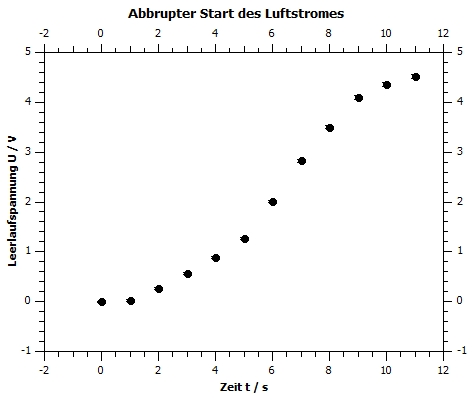
\includegraphics[width=0.6\linewidth]{nudes/wind start.jpg}
    \caption{Leerlaufspannung $U_{leer}$ der Windkraft bei abbrupten Start des Luftstromes pro Sekunde.}
    \label{fig:windkraft start diagramm}
\end{figure}

\noindent
Bei hinzugefügten Kondensator lässt sich ein ähnlicher Anstieg/Abfall der Leerlaufspannung $U_{leer}$ erkennen. 

\begin{figure}[H]
    \centering
    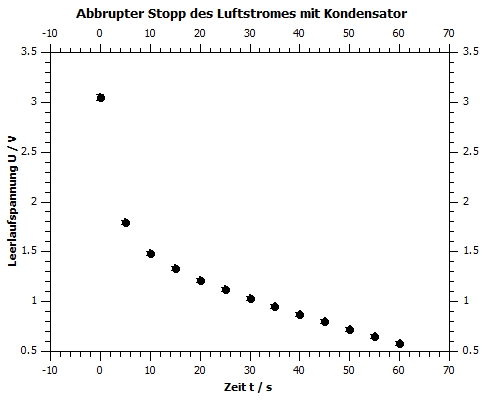
\includegraphics[width=0.6\linewidth]{nudes/wind kondensator stopp.jpg}
    \caption{Leerlaufspannung $U_{leer}$ der Windkraft bei abbrupten Stopp des Luftstromes pro Sekunde mit zugeschaltetem Kondensator.}
    \label{fig:windkraft stopp kondensator diagramm}
\end{figure}


\begin{figure}[H]
    \centering
    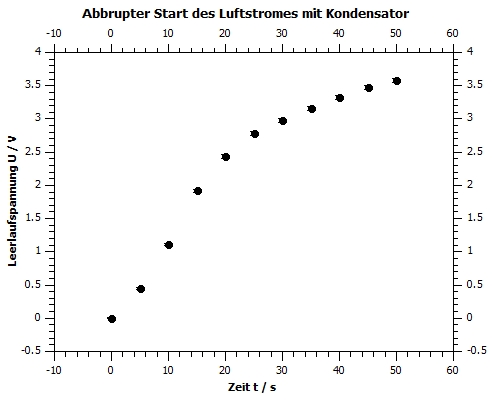
\includegraphics[width=0.6\linewidth]{nudes/wind kondensator start.jpg}
    \caption{Leerlaufspannung $U_{leer}$ der Windkraft bei abbrupten Start des Luftstromes pro Sekunde mit zugeschaltetem Kondensator.}
    \label{fig:windkraft start kondensatordiagramm}
\end{figure}

\noindent
Aus den obigen Graphen wird die Zeitkonstante $t$ über einen exponentiellen Fit (rote Kurve) ermittelt. Dabei ergeben sich folgende Werte: 

\begin{itemize}
    \item Start ohne Kondensator: $t = (8.4 \pm 2.3)s$
    \item Stopp ohne Kondensator: $t = (4.41 \pm 0.4)s$
    \item Start mit Kondensator: $t = (1.0 \pm 26.9)s$
    \item Stopp mit Kondensator: $t = (0.2 \pm 2.4)s$
\end{itemize}

\noindent
Der letzte Teil verwendet die erzeugte Spannung des Windrades als Spannungsquelle für die Brennstoffzelle. Die Zelle speichert die Energie als chemisches Potential, indem Wasserstoff und Sauerstoff erzeugt wird. 
Laut den Messdaten erzeugt die Zelle in $(256.5 \pm 0.1)s$ $(4 \pm 1)ml$ Wasserstoff und $(2 \pm 1)ml$ Sauerstoff. 
Eingesetzt in die Formel \ref{eq:prominute} sieht man, dass die Brennstoffzelle pro Minute eine Wasserstoffmenge von $(1.0 \pm 0.3)ml$ und eine Sauerstoffmenge von $(0.5 \pm 0.3)ml$ erzeugt. 

\section{Diskussion} %diskussion der Unsicherheiten und Ergebnisse und evtl. verlgeich mit Literatur ------------------------------
Anmerkung, in einigen Diagrammen sind die Unsicherheitsbalken teilweise nicht erkennbar, weil die Unsicherheiten teilweise sehr klein sind. 

\subsection{Photovoltaik}
Die Photovoltaik revolutionierte die Energieherstellung. Alles was dafür benötigt war, ist eine Solarzelle und gutes Wetter. Die Energie der Sonne kann zur Stromerzeugung genutzt werden. 
Möglich mach dies der photoelektrische Effekt, welcher von dem bekannten Physiker Albert Einstein gedeutet wurde \cite{wiki1}. Dieser erhielt dafür auch den Nobelpreis im Jahre 1921 \cite{wiki2}. 
\\
\\
In dem Experiment Photovoltaik wird gemessen, wie sich die Spannung und der Strom in verschiedenen Schaltungen verhalten. 
Dabei ist zu beobachten, dass sich bei einer Seriellschaltung die Spannung verdoppelt und bei einer Parallelschaltung der Strom. 
\\
Bei der Strommessung (Diagramm \ref{fig:diagramm Photovoltaik I-d}) ist zu erkennen, dass bei geringsten Abstand nicht der höchste Strom gemessen wurde. 
Dies kann verschiedene Gründe zufolge haben. Zu einem kann die Zelle überhitzen, da die Lichtquelle auch Wärmeenergie abstrahlt, es könnte aber auch die Lichtintensität zu hoch für dieses Solarmodul sein. 
Es gibt einen Punkt, wo zuviel Licht negative Auswirkungen auf die Solarzelle hat. Laut dem Diagramm \ref{fig:diagramm Photovoltaik I-d} ist dieser Punkt bei einen Abstand kleiner als 5cm. Der optimale Abstand liegt laut dem Diagramm zwischen 10 und 15 cm. 
\\
\\
Es lässt sich jedoch auf eine fehlerfreie Durchführung schließen. 

\subsection{Brennstoffzelle}
Brennstoffzellen gewinnen immer mehr an Popularität. Besonders Autos, welche über Brennstoffzellen betrieben werden haben einen hohen Wert in der aktuellen Forschung. 
\\
\\
In diesem Experiment wird eine Brennstoffzelle als Elektrolyse betrieben um Strom zu erzeugen, sowohl auch als kalter Verbrenner um Wasserstoff und Sauerstoff herzustellen. 
Bei der Elektrolyse ist zu beobachte, je höher die Eingangsspannung ist, umso schneller wird Wasserstoff und Sauerstoff erzeugt und umso höher der Strom. 
Dabei wird elektrische Energie in chemische Energie umgewandelt. 
\\
\\
Im zweiten Teil wird aus der vorhandenen chemischen Energie elektrische Energie erzeugt. 
Dadurch lässt sich der Wirkungsgrad bestimmen. Eine Brennstoffzelle besitzt einen Wirkungsgrad von 35-62\% \cite{wiki3}, was auch in diesem Experiment das Ergebnis ist. 
\\
Es lässt sich daher auf eine fehlerfreie Durchführung schließen. 

\subsection{Windkraft}
Windkraft nutzt die Energie des Windes um elektrische Energie zu erzeugen. Dabei werden die Flügel des Windrades Tragflächenförmig angeordnet. 
Durch diese Form entstehen unterschiedliche Strömungsgeschwindigkeiten, wie in Abbildung \ref{fig:tragfläche} der Grundlagen ersichtlich ist. 
\\
\\
Bei diesem Versuch wird gezeigt, dass je stärker der Wind, desto stärker der Energieoutput des Windrades. Laut der Tabelle \ref{tab:Messdaten Windkraft stationär} sieht man mit steigender Eingangsspannung, also ein stärkerer Wind, einen linear ansteigenden Energieoutput. 
Auch wie in Tabelle \ref{tab:Messdaten Windkraft mit d} gezeigt wird, nimmt die Leistung mit zunehmenden Abstand zur Windmaschine annähernd linear ab. 
\\
\\
Bei abbrupten Stoppen des Luftstromes kommt es durch die Drehimpulserhaltung nicht sofort zu einem stopp der Energieerzeugung, sondern erst nach gewisser Zeit. Dies lässt sich auch bei zugeschaltenem Kondensator beobachten. 
Auch bei abbrupten Starten des Luftstromes läuft das Windrad nicht sofort auf maximalem Energieoutput, erst nach gewisser Zeit. 
\\
\\
Es lässt sich auf eine Fehlerfreie Durchführung schließen. 

\section{Zusammenfassung} %klare, übersichtliche vollständige beantwortung der Aufgabenstellung ------------------------------
\subsection{Photovoltaik}

\begin{figure}[H]
    \centering
    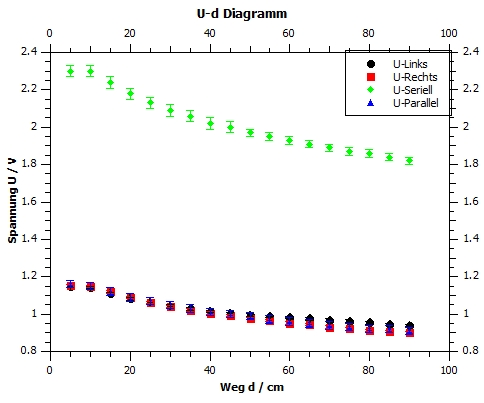
\includegraphics[width=0.6\linewidth]{nudes/u-d diagramm.jpg}
    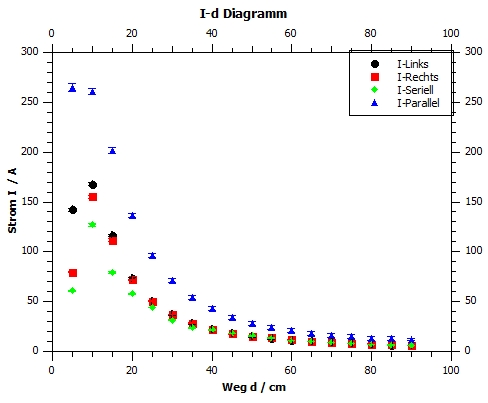
\includegraphics[width=0.6\linewidth]{nudes/i-d diagramm.jpg}
    \caption{Diagramme der Spannung $U$ und Stromstärke $I$ in Abhängigkeit des Abstands $d$.}
    \label{fig:zusammenfassung Photovoltaik}
\end{figure}

\subsection{Brennstoffzelle}

\begin{figure}[H]
    \centering
    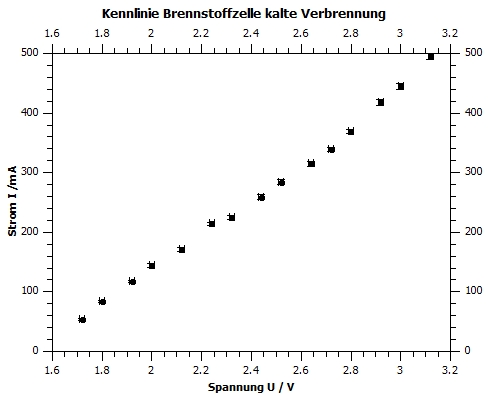
\includegraphics[width=0.6\linewidth]{nudes/brennstoff diagramm i-u.jpg}
    \caption{Diagramm der Brennstoffzelle. Kennlinie bei kalter Verbrennung.}
    \label{fig:zusammenfassung Brennstoffzelle kennlinie verbrennung}
\end{figure}

\begin{itemize}
    \item $P = (0.10 \pm 0.02)W$
    \item $E = (3.7 \pm 1.3)J$ 
    \item $\eta = (60.6 \pm 40.1)\%$
\end{itemize}

\begin{figure}[H]
    \centering
    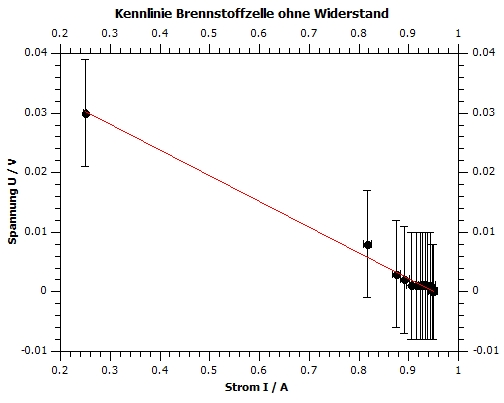
\includegraphics[width=0.6\linewidth]{nudes/brennstoff diagramm ohne r.jpg}
    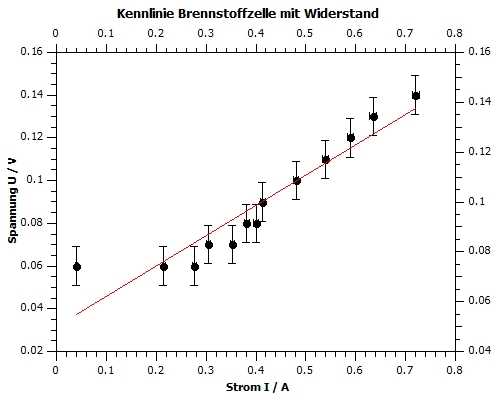
\includegraphics[width=0.6\linewidth]{nudes/brennstoff diagramm mit r.jpg}
    \caption{Kennlinie der Brennstoffzelle bei Elektrolyse mit und ohne Widerstand.}
    \label{fig:zusammenfassung Brennstoffzelle Widerstand}
\end{figure}

\begin{figure}[H]
    \centering
    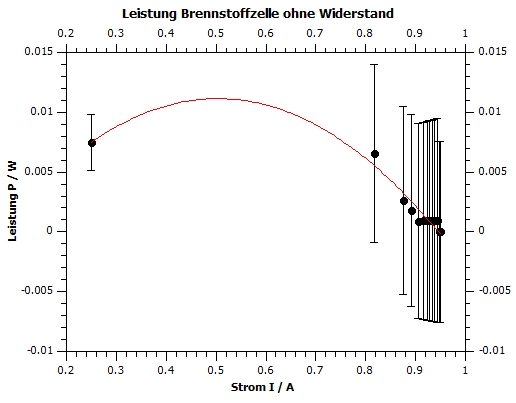
\includegraphics[width=0.6\linewidth]{nudes/brennstoff leistung ohne r.jpg}
    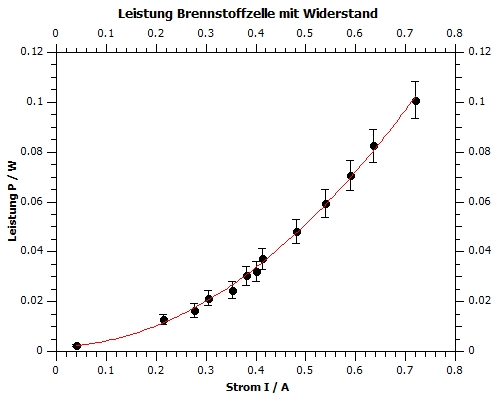
\includegraphics[width=0.6\linewidth]{nudes/brennstoff leistung mit r.jpg}
    \caption{Leistung der Brennstoffzelle bei Elektrolyse mit und ohne Widerstand.}
    \label{fig:zusammenfassung Brennstoffzelle Leistung}
\end{figure}

\subsection{Windkraft}
\begin{figure}[H]
    \centering
    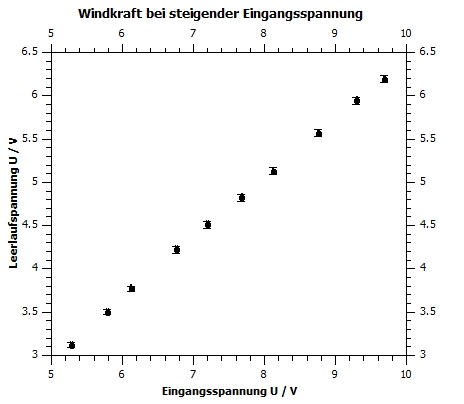
\includegraphics[width=0.6\linewidth]{nudes/wind spannung.jpg}
    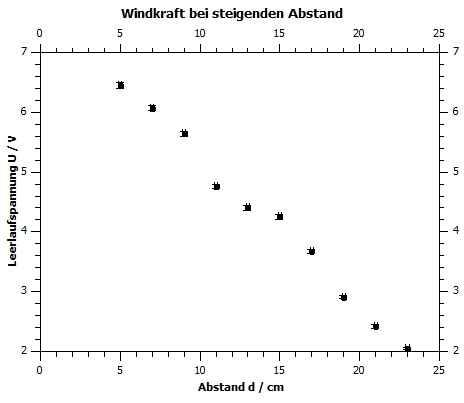
\includegraphics[width=0.6\linewidth]{nudes/wind abstand.jpg}
    \caption{Windkraft bei steigender Eingangsspannung $U_{ein}$ und bei steigendem Abstand $d$. }
    \label{fig:zusammenfassung Windkraft steigend und fallend}
\end{figure}

\begin{figure}[H]
    \centering
    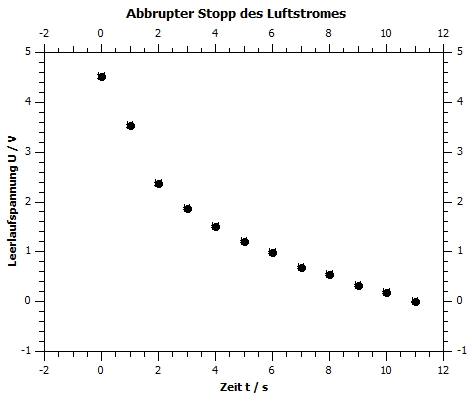
\includegraphics[width=0.6\linewidth]{nudes/wind stopp.jpg}
    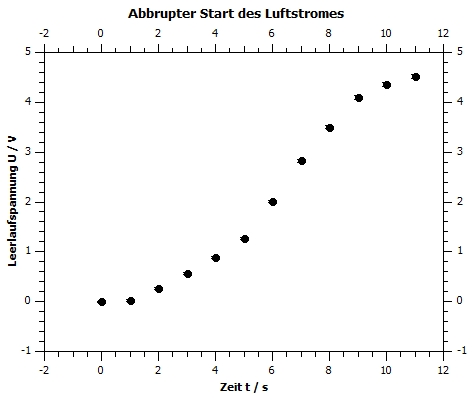
\includegraphics[width=0.6\linewidth]{nudes/wind start.jpg}
    \caption{Leerlaufspannung $U_{leer}$ bei abbrupten Stopp/Start ohne Kondensator}
    \label{fig:zusammenfassung Windkraft stopp start ohne}
\end{figure}

\begin{figure}[H]
    \centering
    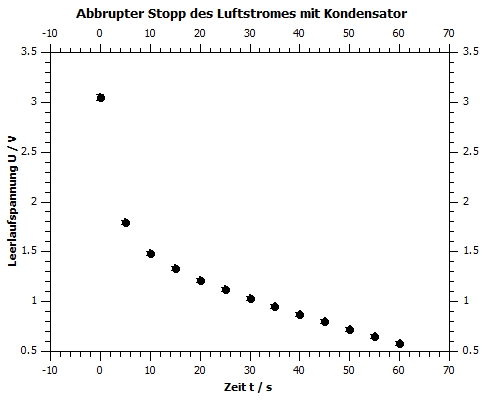
\includegraphics[width=0.6\linewidth]{nudes/wind kondensator stopp.jpg}
    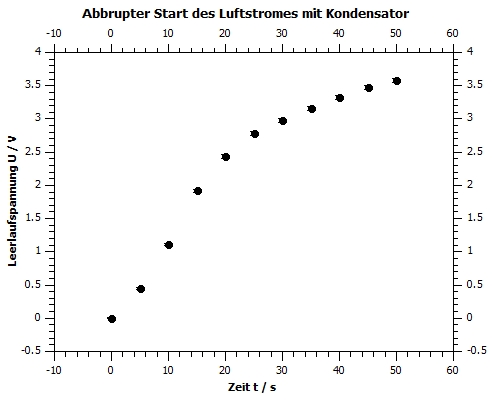
\includegraphics[width=0.6\linewidth]{nudes/wind kondensator start.jpg}
    \caption{Leerlaufspannung $U_{leer}$ bei abbrupten Stopp/Start mit Kondensator}
    \label{fig:zusammenfassung Windkraft stopp start mit}
\end{figure}

Zeitkonstanten bei 

\begin{itemize}
    \item Start ohne Kondensator: $t = (8.4 \pm 2.3)s$
    \item Stopp ohne Kondensator: $t = (4.41 \pm 0.4)s$
    \item Start mit Kondensator: $t = (1.0 \pm 26.9)s$
    \item Stopp mit Kondensator: $t = (0.2 \pm 2.4)s$
\end{itemize}

\begin{itemize}
    \item Erzeugte Wasserstoffmenge pro Minute: $(1.0 \pm 0.3)ml$
    \item Erzeugte Sauerstoffmenge pro Minute: $(0.5 \pm 0.3)ml$
\end{itemize}

\printbibliography[heading=bibintoc]
\end{document}
